\documentclass[10pt]{amsart}
\usepackage[a4paper,margin=22mm]{geometry}
\usepackage[no-math]{fontspec}
\setmainfont{Latin Modern Roman}[SmallCapsFont={lmromancaps10-regular.otf}]
\usepackage{amsmath,amssymb,amsthm,mathtools,hyperref,graphicx,etoolbox}
\providecommand{\Bar}{\overline}
\emergencystretch=3em
\allowdisplaybreaks
\newtheorem{theo}{Theorem}[section]
\newtheorem{lemm}[theo]{Lemma}
\newtheorem{prop}[theo]{Proposition}
\newtheorem{coro}[theo]{Corollary}
\theoremstyle{definition}
\newtheorem{defi}[theo]{Definition}
\newtheorem{rema}[theo]{Remark}
\newtheorem{exam}[theo]{Example}
\numberwithin{equation}{section}
\numberwithin{figure}{section}
\usepackage{tikz}
%\usepackage{thmtools}

\usepackage[labelformat=simple]{subcaption}
    \renewcommand\thesubfigure{$\MK$(\alph{subfigure})}


\usetikzlibrary{patterns,patterns.meta,arrows.meta,
calc,3d,perspective,fadings,shadows,cd}


\newcommand{\bigslant}[2]{{\raisebox{.2em}{$#1$}\left/\raisebox{-.2em}{$#2$}\right.}}
\newcommand{\arr}{\buildrel{\pm 1}\over{\longrightarrow}}
% \arrow[r,"\pm 1" above]
\newcommand{\C}{\mathbb{C}}
\newcommand{\R}{\mathbb{R}}
\newcommand{\Q}{\mathbb{Q}}
\newcommand{\Z}{\mathbb{Z}}
\newcommand{\N}{\mathbb{N}}
\newcommand{\T}{\mathbb{T}}
\newcommand{\F}{\mathbb{F}}
\newcommand{\bbP}{\mathbb{P}}
\renewcommand{\P}{\mathrm{P}}
\renewcommand{\t}{\mathfrak{t}}
\DeclareMathOperator{\Sed}{Sed}

\DeclareMathOperator{\Sd}{Sd}
\DeclareMathOperator{\codim}{codim}
\DeclareMathOperator{\vol}{vol}
\DeclareMathOperator{\rk}{rk}
\DeclareMathOperator{\Res}{Res}
\DeclareMathOperator{\card}{card}
\DeclareMathOperator{\coker}{coker}
\DeclareMathOperator{\Hom}{Hom}
\DeclareMathOperator{\id}{id}
\DeclareMathOperator{\Tor}{Tor}
\DeclareMathOperator{\df}{d}
\DeclareMathOperator{\convhull}{Conv.Hull}
\DeclareMathOperator{\Conv}{Conv}

\newcommand{\Cell}{\mathbf{Cell}}
\newcommand{\Mod}{\mathbf{Mod}}
\newcommand{\Fbar}{\hat{F}}
\newcommand{\Hbar}{\hat{H}}
\newcommand{\ibar}{\hat{\imath}}
\newcommand{\smallslant}[2]{{#1}/{#2}}
\newcommand{\ori}{[\t(\Z)]}


\newenvironment{alcases}{\left\{\begingroup\arraycolsep=0pt\renewcommand{\arraystretch}{1.2}\begin{array}{r@{\;}l@{\quad}l}}{\end{array}\endgroup\right.}
%%%%%%%%%%%%%%%%%%%%%%%%%%%%%%%%%%%%%%%%%%%%%%%%%%%%%%%%%%%%%%%%%%%%%%%%%%%%%%%%%%%%%%%%%%%%%%%%%%%%%%%%%%%%%%%%%%%%%%%%%%%%
\graphicspath{{./figures/}}

\newcommand*{\mk}{\mkern -1mu}
\newcommand*{\Mk}{\mkern -2mu}
\newcommand*{\mK}{\mkern 1mu}
\newcommand*{\MK}{\mkern 2mu}

%\hypersetup{urlcolor=purple, linkcolor=blue, citecolor=red}

\newcommand*{\romanenumi}{\renewcommand*{\theenumi}{\roman{enumi}}}
\newcommand*{\Romanenumi}{\renewcommand*{\theenumi}{\Roman{enumi}}}
\newcommand*{\alphenumi}{\renewcommand*{\theenumi}{\alph{enumi}}}
\newcommand*{\Alphenumi}{\renewcommand*{\theenumi}{\Alph{enumi}}}
\let\oldtilde\tilde
\renewcommand*{\tilde}[1]{\mathchoice{\widetilde{#1}}{\widetilde{#1}}{\oldtilde{#1}}{\oldtilde{#1}}}
\let\oldhat\hat
\renewcommand*{\hat}[1]{\mathchoice{\widehat{#1}}{\widehat{#1}}{\oldhat{#1}}{\oldhat{#1}}}
\let\oldexists\exists
\renewcommand*{\exists}{\mathrel{\oldexists}}
\let\oldforall\forall
\renewcommand*{\forall}{\mathrel{\oldforall}}
%%%%%%%%%%%%%%%%%%%%%%%%%%%%%%%%%%%%%%%%%%%%%%%%%%%%%%%%%%%%%%%%%%%%%%%%%%%%%%%%%%%%%%%%%%%%%%%%%%%%%%%%%%%%%%%%%%%%%%%%%%%%
\title[Cellular Poincaré--Lefschetz duality]{Cellular Poincaré--Lefschetz duality for finite dimensional locally finite regular CW dihomologic cosheaves with one-degree local homology}
\author{Jules Chenal}
\date{Annales Henri Lebesgue8(2025),277–327; DOI10.5802/ahl.236}
\hypersetup{hidelinks}
\begin{document}
\maketitle
\setcounter{section}{1}
\section{CW-Complexes and Cellular Homology}

CW-complexes were introduced by J.~H.~C.~Whitehead in \emph{Combinatorial homotopy.~{I}}, \cite{Whi_com_hom}. Their underlying topological spaces, their \emph{supports}, form a broad family of spaces usually considered well-behaved. Some of the sheaves defined on their support are particularly adapted to their structure. They can be described by a relatively small amount of data and their cohomology can be computed by the techniques of cellular cohomology. In the following paragraphs we give a succinct presentation of the objects at play in this text.

\subsection{CW-Complexes}

\begin{defi}[CW-Complex]
A \emph{CW-complex} $K$ is the data of a Hausdorff topological space $|K|$, called the \emph{support} of $K$, filtered by closed subsets $\varnothing=K^{(-1)}\subset K^{(0)}\subset\dots\subset K^{(k)}\subset\dots\subset |K|$ called the \emph{skeleta} of $K$ whose union covers $|K|$. Such filtration has to satisfy the additional properties:
\begin{enumerate}
\item For every $k\geq 0$ and every connected component $e^k$ of $ K^{(k)}\setminus K^{(k-1)}$, called an \emph{open $k$-cell}, there exists a surjective continuous map from the closed\linebreak $k$-dimensional ball onto the closure $\bar{e}^k$ that carries homeomorphically the open ball onto $e^k$, such a map is called a \emph{characteristic map} of the open cell~$e^k$;
\item $|K|$ has the weak topology: \emph{a subset $A\subset |K|$ is closed if and only if its intersection~$A\cap\Bar{e}^k$ with every closed cell is closed};
\item Every skeleton $K^{(k)}$ has the weak topology in the same sense as in point 2.
\end{enumerate}
We call the dimension of $K$, $\dim K$, the smallest integer from which the filtration $(K^{(k)})_{k\,\geq\,-1}$ is stationary. It might be $\infty$. A \emph{sub-complex} $L$ of $K$ is determined by a closed subset $|L|$ for which the induced filtration:
\begin{equation*}
\varnothing=L^{(-1)}\subset L^{(0)}\subset\dots\subset L^{(k)}\subset\dots\subset |L| \textnormal{ where }L^{(k)}:=|L|\cap K^{(k)} \textnormal{ for all }k\in \N,
\end{equation*}
turns it into a CW-complex of its own right. The intersection of some sub-complexes is again a sub-complex. For all subsets $A$ of $|K|$ we set $K(A)$ to be the smallest sub-complex containing $A$ in its support i.e. the intersection of all the sub-complexes containing $A$ in their support.
\end{defi}

\begin{defi}[Simplicial Complex]\label{def:simplicial_cpx}
A \emph{simplicial complex} $S$ is a collection~$V$ of \emph{vertices} and a collection $T$ of finite subsets of $V$, called \emph{simplices}, such that:
\begin{equation*}
\forall \sigma\in T,\; \tau\subset\sigma \Rightarrow \tau\in T.
\end{equation*}
The \emph{geometric realisation} of $S$ is the set:
\begin{equation*}
\bigcup_{\sigma\,\in\,T} \convhull(v\in\sigma) \subset \bigoplus_V\R,
\end{equation*}
with the induced product topology.
\end{defi}

\begin{exam}
The most basic examples (of CW-complexes) are given by simplices and all the geometric realisations of simplicial complexes as defined in~\cite{Whi_sim_spa}, c.f. Definition~\ref{def:simplicial_cpx}. More generally, a polyhedral complex is an example of CW-complex. By a polyhedral complex we mean a collection $K$ of polytopes\footnote{A convex hull of a finite number of vertices.} in a real vector space that contains all the faces of its polytopes and in which two distinct polytopes intersect on a common face (which might be empty). In a polyhedral complex the open cell corresponding to a polytope is its \emph{relative interior}, that is to say, the topological interior of the polytope in the affine space it spans.
\end{exam}
\begin{exam}
Some extremely classical examples are given by the real projective spaces. They filter themselves ${\R \P^0\subset\R \P^1\subset\dots \subset \R \P^n}$ by inclusion on the first coordinates. The induced partition of $\R \P^n$ into open cells corresponds to a decomposition into affine spaces, one for every $0\leq k\leq n$. By extension, the inductive limit $\R \P^\infty$ is also a CW-complex for the induced filtration.
\end{exam}

\begin{defi}
A CW-complex in which every point has a neighbourhood that meets only finitely many open cells is called \emph{locally finite}.
\end{defi}

Any \emph{finite} (with finitely many cells) CW-complex is obviously locally finite. Among our examples, $\R \P^\infty$ is not locally finite as the neighbourhood of a point in the open cell $\R^k$ will meet all the open cells $\R^n$ for all $n\geq k$.

\begin{prop}[{\cite[(G), pp.~225-227, (M), pp.~230-231]{Whi_com_hom}}]
A CW-complex is a normal and locally contractible topological space.
\end{prop}

\begin{defi}
A \emph{regular} CW-complex is one that admits for each cell a characteristic map that is a homeomorphism over the entire closed ball.
\end{defi}

In particular, every closed cell of a regular CW-complex is homeomorphic to a closed ball. It excludes the CW-complex structure of the real projective spaces (apart from the trivial case $\R \P^0$) given by affine spaces as every positive dimensional closed cell is a projective space, different from a closed ball. An important example of regular CW-complex is given by geometric realisations of simplicial complexes in which every closed cell is a closed simplex, hence topologically a closed ball. Likewise, a polyhedral complex is necessarily a regular CW-complex.

%\vspace{5pt}

Given a general CW-complex, the formula $e_1\leq e_2\iff \Bar{e}_1\subset\Bar{e}_2$ defines an order on its cells. When the CW-complex is regular this order shares the same properties as the inclusion of faces in a simplicial complex.

\begin{lemm}
For any two open cells $e_1,e_2$ of $K$, a regular CW-complex, $e_1$ meets the closure of $e_2$ if and only if it is fully contained in it:
\begin{equation*}
e_1\cap\Bar{e}_2\neq \varnothing \, \iff\, e_1\subset \Bar{e}_2.
\end{equation*}
\end{lemm}

One can find a proof in~\cite[pp.~229-230, R.R.1]{Coo-Fin_hom_cel}.
Therefore, in a regular CW-complex, whenever a cell $e_1$ meets the closure of another one $e_2$ we have $e_1\leq e_2$ and we say that $e_1$ is a \emph{face} of $e_2$. If $e_1$ is distinct from $e_2$ we say that $e_1$ is a \emph{proper face} of $e_2$ and denote it by $e_1<e_2$. Furthermore, if $e_1\leq e_2$ or $e_2\leq e_1$ we say that $e_1$ and $e_2$ are \emph{adjacent}.

\begin{lemm}
Let $K$ be a regular CW-complex. For all cells $e$ of $K$, the support of the sub-complex $K(e)$ is the closure $\bar{e}$.
\end{lemm}

\begin{lemm}\label{lemm:2_faces}
Let $k\in\N$ and $e^{k+2}$ be an open cell of a regular CW-complex $K$. For all faces of codimension~2, $e^k$ of $e^{k+2}$ there are exactly two cells of codimension~1 between $e^k$ and $e^{k+2}$:
\begin{equation*}
\card \left\{e^{k+1}\,\middle|\,e^k<e^{k+1}<e^{k+2}\right\}=2.
\end{equation*}
\end{lemm}

\begin{lemm}[Open Star]
Let $e$ be a cell of a regular CW-complex $K$. The union of all the cells having $e$ as a face, called the \emph{open star} of $e$, is an open subset of $|K|$.
\end{lemm}

Proofs of these statements are given in~\cite[Proposition~1.6, p.~30, Theorem~4.2, pp.~231-232, Lemma~4.1, p.~230]{Coo-Fin_hom_cel}.
%\footnote{Ibid. in order, .}
In a locally finite CW-complex $K$, the open star of a cell is a finite union of cells, so its closure, the \emph{closed star} of the cell, is a finite sub-complex of $K$. The collection $K-e$ of all the cells whose closure avoids $e$ is the complement of the open star of $e$ and is a sub-complex of $K$. Its underlying topological space is a deformation retract of $|K|\setminus e$ and is the largest sub-complex of $K$ contained in the complement $|K|\setminus e$. For all subsets $A$ of $|K|$, we denote by $K-A$ the largest sub-complex of $K$ contained in $|K|\setminus A$.

\begin{defi}[Subdivisions]
A \emph{subdivision} $K'$ of a CW-complex $K$ is a CW-complex on the same support $|K'|=|K|$ in which every cell $e'\in K'$ is contained in a cell $e\in K$. Another way of saying it is that the partition of $|K|$ into open cells of $K'$ is finer than the partition given by the open cells of $K$.
\end{defi}

\begin{figure}[h]
\centering
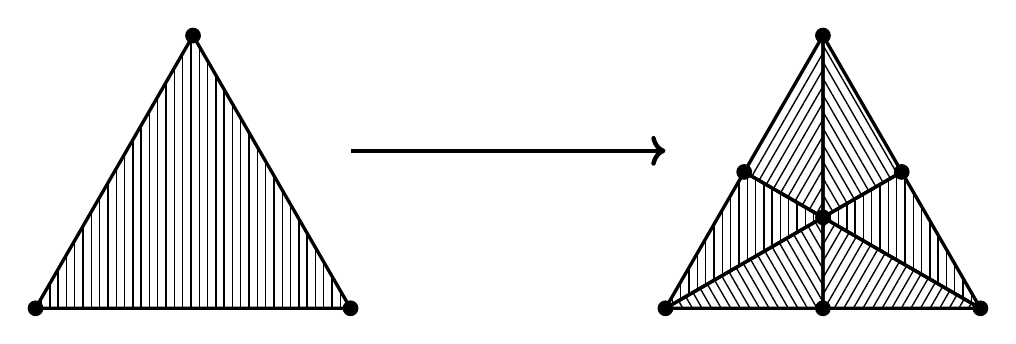
\begin{tikzpicture}[scale=2]
\tikzfading[name=fade inside, inner color=transparent!100, outer color=transparent!50]
\coordinate (a) at (0,0);
\coordinate (b) at (2,0);
\coordinate (c) at ($(a)+(60:2)$);
\coordinate (a1) at ($(a)+(4,0)$);
\coordinate (b1) at ($(b)+(4,0)$);
\coordinate (c1) at ($(c)+(4,0)$);
\coordinate (center) at ($(a)!0.33333333!(a1)+(a)!0.33333333!(b1)+(a)!0.33333333!(c1)$);
\fill[pattern={Lines[angle=90, line width=.5pt]}] (a) -- (b)-- (c) -- cycle;
\draw[very thick](a) -- (b)-- (c) -- cycle;
\draw[very thick] (a1) -- (b1)-- (c1) -- cycle;
\filldraw[pattern={Lines[angle=90, line width=.5pt]},very thick] (a1) -- (center) -- ($(c1)!(b1)!(a1)$);
\filldraw[pattern={Lines[angle=120, yshift=-3.75pt, line width=.5pt]},very thick] (a1) -- (center) -- ($(b1)!(c1)!(a1)$);
\filldraw[pattern={Lines[angle=60, yshift=0.75pt, line width=.5pt]},very thick] (b1) -- (center) -- ($(b1)!(c1)!(a1)$);
\filldraw[pattern={Lines[angle=90, line width=.5pt]},very thick] (b1) -- (center) -- ($(b1)!(a1)!(c1)$);
\filldraw[pattern={Lines[angle=120, yshift=5pt, line width=.5pt]},very thick] (c1) -- (center) -- ($(c1)!(a1)!(b1)$);
\filldraw[pattern={Lines[angle=60, yshift=4pt, line width=.5pt]},very thick] (c1) -- (center) -- ($(c1)!(b1)!(a1)$);
\fill (a) circle (.05);
\fill (a1) circle (.05);
\fill (b) circle (.05);
\fill (b1) circle (.05);
\fill (c) circle (.05);
\fill (c1) circle (.05);
\fill ($(a1)!.5!(b1)$) circle (.05);
\fill ($(c1)!.5!(b1)$) circle (.05);
\fill ($(a1)!.5!(c1)$) circle (.05);
\fill (center) circle (0.05);
\draw[->,ultra thick] ($(b)+(0,1)$) -- ($(a1)+(0,1)$);
\end{tikzpicture}
\caption{The barycentric subdivision of the triangle.}\label{fig:bar_trig}
\end{figure}

A common example of subdivision is given by the \emph{barycentric subdivision} $\Sd S$ of a simplicial complex $S$, see for instance Figure~\ref{fig:bar_trig}. It is described abstractly as follows: the vertices of $\Sd S$ are given by the simplices of $S$ and the simplices of $\Sd S$ by the flags of simplices of $S$. More concretely, a collection of simplices $\{\sigma_0,\dots,\sigma_k\}$ is a simplex of $\Sd S$ if and only if it can be totally ordered i.e. there is a permutation $\pi$ of the indices $\{0,\dots,k\}$ such that:
\begin{equation*}
\sigma_{\pi(0)} <\dots < \sigma_{\pi(n)}.
\end{equation*}
One can define a homeomorphism between the geometric realisation of $\Sd S$ and the geometric realisation of $S$ by sending each vertex of $\Sd S$ to the barycenter of its corresponding simplex in $S$ and extending this map by linearity. An example is depicted in Figure~\ref{fig:homeo_segment}.
\begin{figure}[h]
\centering
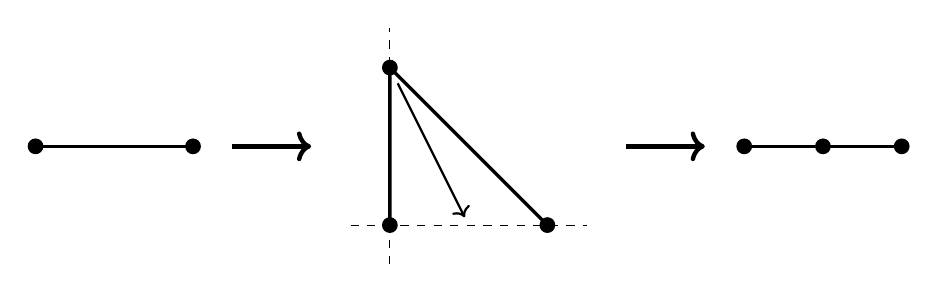
\begin{tikzpicture}[scale=2]
\draw[very thick] (0,0) -- (1,0);
\fill (0,0) circle (0.05);
\fill (1,0) circle (0.05);
\draw[->,ultra thick] (1.25,0) -- (1.75,0);
\draw[dashed] (2,-.5) -- (3.5,-.5);
\draw[dashed] (2.25,-.75) -- (2.25,.75);
\fill (2.25,-.5) circle (0.05);
\fill (3.25,-.5) circle (0.05);
\fill (2.25,.5) circle (0.05);
\draw[very thick] (2.25,-.5) -- (2.25,.5) -- (3.25,-.5);
\draw[thick,->] ($(2.25,.5)!.1!(2.75,-.5)$) -- ($(2.25,.5)!.95!(2.75,-.5)$);
\draw[->,ultra thick] (3.75,0) -- (4.25,0);
\draw[very thick] (4.5,0) -- (5.5,0);
\fill (4.5,0) circle (0.05);
\fill (5,0) circle (0.05);
\fill (5.5,0) circle (0.05);
\end{tikzpicture}
\caption{The homeomorphism from the barycentric subdivision of the segment to the initial segment.}\label{fig:homeo_segment}
\end{figure}

The image of the skeletal filtration of $\Sd S$ under this homeomorphism defines a subdivision of the CW-complex induced by $S$ in the sense of the previous definition. Note that if instead we chose to send each vertex of $\Sd S$ to an arbitrary point in the open cell defined by the corresponding simplex in $S$ (and then extending the map by linearity) we would also have defined a subdivision of $S$ that is equivalent, in a combinatorial way, to the previous one. We could say that the barycentric subdivision is only defined unequivocally on the abstract level. The same abstract procedure can be performed with a regular CW-complex $K$. The \emph{barycentric subdivision} $\Sd K$ of $K$ is defined to be the following simplicial complex:
\begin{enumerate}
\item Every cell of $K$ corresponds to a vertex of $\Sd K$;
\item A finite set of cells of $K$ corresponds to a simplex of $\Sd K$ if and only if it is totally ordered by adjacency.
\end{enumerate}

\begin{prop}\label{prop:bar_sub_cw}
Let $K$ be a regular CW-complex. The geometric realisation of $\Sd K$ is homeomorphic to $|K|$ in such a way that $\Sd K$ can be seen as a subdivision of $K$.
\end{prop}

This proposition, proven in~\cite[Theorem~1.7, pp.~80-81.]{Lun-Wei_top_cw},
%\footnote{A. Lundell and S. Weingram. \emph{The Topology of CW Complexes}, } 
allows us to see a regular CW-complex as ``a simplicial complex in which the simplexes are more efficiently combined into closed cells.''\footnote{Ibid. p.~77.} Another feature of simplicial complexes shared by regular complexes is the following:

\begin{prop}
In a regular CW-complex the open stars of cells are contractible.
\end{prop}

\begin{proof}
The geometric realisation of $\Sd K$ lives in the real vector space $V$ spanned by the cells of $K$. We use the same symbol to denote a cell $e^k$ and its associated generator in $V$. Hence, an element of $V$ is a formal finite linear combination of the cells of $K$. We endow this vector space with the norm $1$:
\begin{equation*}
\left\|\sum_{e\,\in\,K} x_ee\right\|_1=\sum_{e\,\in\,K}|x_e|.
\end{equation*}
The geometric realisation $|\Sd K|$ is the union of the convex hulls of the sets of cells $\{e^{k_0},\dots,e^{k_n}\}$ corresponding to barycentric simplices i.e. flags of cells. It is a subset of the intersection of the unit sphere with the positive ortant $V_+:=\{\sum_{e\,\in \,K}x_ee\in V\;|\;x_e\geq 0\}$. For a flag of cells $e^{k_0}<\dots<e^{k_n}$ let us denote here the corresponding open simplex by:
\begin{equation*}
\big(e^{k_0};\dots\,;e^{k_n}\big):=\left\{\sum_{i=0}^n x_ie^{k_i}\;\middle|\;\forall i,\, x_i>0\text{ and }\sum_{i=0}^n x_i=1\right\}.
\end{equation*}
An open cell $e^k$ of $K$ corresponds under the homeomorphism of Proposition~\ref{prop:bar_sub_cw} to the union of the open barycentric simplices $(e^{k_0};\dots\,;e^{k_n})$ for which $e^{k_n}=e^k$. Therefore, the open star $S$ of $e^k$ is in this context:
\begin{equation*}
S=\bigcup_{\substack{e^{k_0}\,<\,\dots\,<\,e^{k_n}\\e^k\,\leq\,e^{k_n}}}\big(e^{k_0};\dots\,;e^{k_n}\big).
\end{equation*}
We consider the family of bounded linear operators $(\Phi_t:V\rightarrow V)_{0\,\leq\,1\,\leq\,t}$ defined by $\Phi_t=(\id-\pi)+t\pi$, where $\pi$ denotes the projection to the sub-space spanned by the cells that do not contain $e^k$ parallely to the sub-space spanned by those that contain it. Let $U$ be the open set of $V_+$ of vectors that have at least one positive coordinate indexed by a cell that contains $e^k$. We have $S=|\Sd K|\cap U$. For all $t\in[0;1]$, the map:
\begin{equation*}
\begin{array}{rcl}
\Psi:[0;1]\times U& \longrightarrow & U \\%
u & \longmapsto & \frac{\|u\|_1}{\|\Phi_t(u)\|_1}\Phi_t(u)\,,
\end{array}
\end{equation*}
is continuous and every partial map $\Psi(t;-)$ stabilises $S$. The image $\Psi(0;S)$ is the union of the open barycentric simplices $(e^{k_0};\dots\,;e^{k_n})$ for which $e^k\leq e^{k_0}$. Note that the restriction of every map $\Psi(t;-)$ is constant on this set. Therefore $\Psi(0;S)$ is a deformation retract of $S$. Now this set retracts on the barycentre of $e^k$ by simple convex interpolation $(t;u)\in [0;1]\times\Psi(0;S)\mapsto (1-t)u+te^k$, thus $S$ is contractible.
\end{proof}

When we consider the barycentric subdivision of a finite regular CW-complex we increase considerably the number of cells. There is, however, a less expensive procedure that builds a ``pseudo-subdivision'' for any regular CW-complex $K$ that sits between $K$ and $\Sd K$. By pseudo-subdivision we mean a certain recombination of the barycentric simplices that looks a lot like a regular subdivision.

\begin{defi}[Dihomologic Pseudo-subdivision]
Let $K$ be a regular CW-complex. Let $e^p\leq e^q$ be a pair of adjacent cells, we define its associated \emph{dihomologic pseudo-cell} to be the union of the open barycentric simplices\footnote{The open simplex on a vertex set $v_0,\dots,v_n$ is the set
\[
\left\{\sum_{i=0}^nt_iv_i\;\middle|\; \forall i,\,t_i>0\text{ and }\sum_{i=0}^nt_i=1\right\}.
\]
} associated with the flags $e^{k_1}<\dots<e^{k_n}$ for which $e^p= e^{k_1}$ and $e^{k_n}=e^q$. These ``open'' pseudo-cells form a partition of the simplicial complex $\Sd K$. We call such partition the \emph{dihomologic pseudo-subdivision} of $K$. We say that the dihomologic pseudo-cell associated with the pair $e^p\leq e^q$ has dimension $q-p$. Figure~\ref{fig:dih_sub_disc} illustrates this procedure on a disc.
\end{defi}

\begin{figure}[h]
\centering
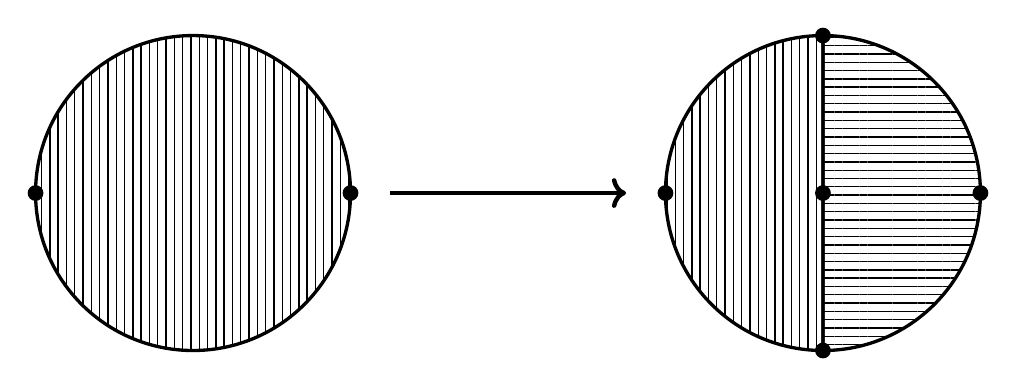
\begin{tikzpicture}[scale=2]
\filldraw[pattern={Lines[angle=90, line width=.5pt]},very thick] (0,0) circle (1);
\fill (-1,0) circle (.05);
\fill (1,0) circle (.05);
\fill (3,0) circle (.05);
\fill (5,0) circle (.05);
\fill (4,1) circle (.05);
\fill (4,-1) circle (.05);
\fill (4,0) circle (.05);
\filldraw[pattern={Lines[angle=90, line width=.5pt, xshift=1pt]},very thick] (4,-1) -- (4,1) arc [start angle=90, end angle=270, radius=1] (4,-1) ;
\filldraw[pattern={Lines[angle=0, line width=.5pt]},very thick] (4,1) -- (4,-1) arc [start angle=270, end angle=450, radius=1] (4,1) ;
\draw[->,ultra thick] (1.25,0) -- (2.75,0);
\end{tikzpicture}
\caption{The dihomologic pseudo-subdivision of a regular CW-complex structure of the disc.}\label{fig:dih_sub_disc}
\end{figure}

As every open dihomologic pseudo-cell is a union of open barycentric simplices their closures are naturally supports of sub-complexes of the barycentric subdivision. We always endow the closed dihomologic pseudo-cell with this particular simplicial structure. The dihomologic pseudo-subdivision shares many properties with a regular subdivision of $K$ but may fail to define a CW-complex structure on $|K|$. We do not know if closures of dihomologic pseudo-cells are always homeomorphic to closed balls. However, for a broad variety of examples as we will see, this is indeed the case and the dihomologic pseudo-subdivision is a regular subdivision of $K$.

\begin{rema}
We chose to use the terminology ``dihomologic'' because Zeeman's dihomology bicomplex, c.f. \cite{Zee_dih_i,Zee_dih_ii,Zee_dih_iii}, would be the cellular chain complex of this pseudo-subdivision. This bicomplex was latter (dually) rediscovered by Forman in~\cite{For_comb_nov} under the name of ``combinatorial differential forms''.
\end{rema}

\begin{defi}[Collapse]
Let $S=(V;T)$ be a simplicial complex.~A \emph{free simplex} of $S$ is a simplex $\sigma\in T$ strictly contained in exactly one maximal simplex of $S$. An \emph{elementary collapse} of $S$ is the operation:
\begin{equation*}
S\mapsto \big(V;T\setminus\{\tau\,:\,\sigma\subset \tau\}\big),
\end{equation*}
where $\sigma$ is a free simplex of $S$. A \emph{collapse} is a composition of elementary collapses. A complex is called \emph{collapsible} if it can be collapsed to a single vertex.
\end{defi}

\begin{prop}
Let $e^p\leq e^q$ be a pair of adjacent cells of $K$. The closure of the pseudo-cell associated with $e^p\leq e^q$, is a collapsible simplicial complex of pure dimension $q-p$. Moreover, any codimension~1 simplex of the open pseudo-cell is exactly contained in two of its maximal simplices.
\end{prop}

\begin{proof}
Let $e^p\leq e^q$ be a pair of adjacent cells. If $e^p=e^q$ the associated pseudo-cell is a single vertex and the statement of the proposition is true. Now suppose $e^p$ is a proper face of $e^q$. The closure of the associated pseudo-cell is the union of the barycentric simplices whose flags $e^{k_1}<\dots<e^{k_n}$ satisfy $e^p\leq e^{k_1}<\dots<e^{k_n}\leq e^q $. This is a simplicial sub-complex of $\Sd K$. A maximal simplex of this closed pseudo-cell is given by a maximal flag of adjacent cells of $K$ starting with $e^p$ and ending with~$e^q$. Since $K$ is regular such flag has necessarily length $q-p+1$, so the corresponding simplex has dimension $q-p$. Hence, the closed pseudo-cell is a pure $(q-p)$-dimensional simplicial complex. If $q-p=1$, this closed pseudo-cell corresponds to the closed barycentric edge $e^p<e^q$. This is a collapsible complex. If $q-p>1$, the maximal simplices of the closed pseudo-cell correspond to flags $e^p<e^{p+1}<\dots<e^{q-1}<e^q$. They all have a codimension~2 free face, associated with $e^{p+1}<\dots<e^{q-1}$. If we collapse all such simplices we obtain the union of the closed $(q-p-1)$-simplices associated with the flags of the form $e^p<e^{k_1}<\dots<e^{k_{q-p-2}}<e^q$. All such simplices are now maximal and contain each a free face of codimension~2, namely $e^{k_1}<\dots<e^{k_{q-p-2}}$. We can recursively perform such collapses to end up with the barycentric edge $e^p<e^q$. Thus, the closed pseudo-cell of the pair $e^p\leq e^q$ is collapsible. For the final part, a simplex of codimension~1 of the open pseudo-cell is given by a flag $e^p<e^{k_1}<\dots<e^{k_{q-p-2}}<e^q$ of length $q-p$ and has the form $e^p<\dots<e^i<e^{i+2}<\dots<e^q$. Since $K$ is regular there are exactly two $(i+1)$-cells between $e^i$ and $e^{i+1}$, hence two $(q-p)$-simplices.
\end{proof}

\begin{prop}
The open pseudo-cell associated with the pair $e^p\leq e^q$ meets the closed pseudo-cell indexed by the pair $e^{p'}\leq e^{q'}$ if and only if $e^{p'}\leq e^{p}$ and $e^q\leq e^{q'}$. This means that every open barycentric simplex of the former is contained in the latter. Moreover, if $\epsilon_0$ is an open pseudo-cell of dimension $k$ included in a closed pseudo-cell $\bar{\epsilon}_2$ of dimension $k+2$ then there are exactly two open pseudo-cells $\epsilon_1$ of dimension $k+1$ such that $\epsilon_0\subset\bar{\epsilon}_1$ and $\epsilon_1\subset\bar{\epsilon}_2$.
\end{prop}

\begin{proof}
The first part is a consequence of the definition. For the second part, we choose $\epsilon_0$ corresponding to a pair $e^{p+a}\leq e^{p+a+k}$ and $\epsilon_2$ to a pair $e^p\leq e^{p+a+k+b}$ satisfying $e^p\leq e^{p+a}\leq e^{p+a+k}\leq e^{p+a+k+b}$. By assumption, we have $a+b=2$ and three different cases can occur: one of the two numbers $a,b$ is $2$ and the other $0$ or both equal $1$. The two first cases are symmetric. If it's $a$ that equals $2$ we have $e^p\leq e^{p+2}\leq e^{p+2+k}\leq e^{p+2+k}$ and the two $(k+1)$-pseudo-cells between $\epsilon_0$ and $\epsilon_1$ are those associated with the two pairs $e^{p+1}\leq e^{p+2+k}$ with $e^p\leq e^{p+1}\leq e^{p+2}$. If both $a$ and $b$ equal $1$ then we have $e^p\leq e^{p+1}\leq e^{p+1+k}\leq e^{p+2+k}$ and the two $(k+1)$-pseudo-cells between $\epsilon_0$ and $\epsilon_2$ are those associated with the two pairs $e^p\leq e^{p+1+k}$ and $e^{p+1}\leq e^{p+2+k}$.
\end{proof}

In the light of this property it makes sense to talk about \emph{adjacent} pseudo-cells as we do for cells of regular CW-complexes. As in the regular case, if $\epsilon$ and $\epsilon'$ are adjacent pseudo-cells with $\epsilon\subset\overline{\epsilon}'$ we say that $\epsilon$ is a \emph{face} of $\epsilon'$. If in addition $\epsilon\neq\epsilon'$ we say that $\epsilon$ is a \emph{proper face} of $\epsilon'$. Also we see here that two dihomologic pseudo-cells meet on a common face if their intersection is non-empty. Note that this property might not be true in $K$, two closed cells meet on the union of their common faces if the intersection is non-empty. Let $e^p< e^q$ be a proper adjacent pair of cells of $K$ and $\epsilon$ denote its associated pseudo-cell. The simplicial complex supported on the closure, $(\Sd K)(\epsilon)$, is the join of the barycentric edge $e^p<e^q$ and a sub-complex $A(e^p;e^q)\subset\Sd K$. This sub-complex is the collection of all the barycentric simplices indexed by the flags $e^{k_1}<\dots<e^{k_{n}}$ for which $e^p<e^{k_1}$ and $e^{k_{n}}<e^q$.

\begin{defi}[Homology Manifold]\label{definition:homo_man}
A \emph{homology manifold} of dimension $n\in\N$ is the support $X$ of a regular, finite dimensional, locally finite CW-complex for which the graded local homology group $H_*(X;X\setminus\{x\};\Z)$ of every point $x\in X$ is isomorphic to either $H_*(\R^n;\R^n\setminus \{0\};\Z)$ or $0$. The \emph{boundary} of $X$, denoted by $\partial X$, is the set of points $x\in X$ for which $H_*(X;X\setminus\{x\};\Z)=0$.
\end{defi}

\begin{prop}\label{prp:A_homo}
The support of $A(e^p;e^q)$ is a connected homology manifold of dimension $(q-p-2)$ whose $(p+1)$-fold suspension is homeomorphic to a $(q-1)$-sphere.
\end{prop}

\begin{proof}
Let $B$ denote the simplicial complex $(\Sd K)(\bar{e}^q\setminus e^q)$ and $e^0<\dots<e^p$ be a complete flag of cells of $K$. The simplicial complex $A(e^p;e^q)$ is the link in $B$ of the barycentric simplex associated with $e^0<\dots<e^p$. $B$ is a simplicially triangulated $(q-1)$-sphere thus in application of~\cite[Proposition~1.3 p.~5]{Gal-Ste_Cla_Sim} the $(p+1)$-fold suspension of $A(e^p;e^q)$ is homeomorphic to a $(q-1)$-sphere. The Mayer-Vietoris long exact sequence in singular homology implies that, if $\Sigma A$ is the suspension of a topological space $A$, we have $H_0(\Sigma A;\Z)=\Z$, $H_{k}(\Sigma A;\Z)\cong H_{k-1}(A;\Z) \text{ for all }k\geq 2$ and the exact sequence:
\begin{equation*}
0 \rightarrow H_1(\Sigma A;\Z) \rightarrow H_0(A;\Z) \rightarrow \Z \rightarrow 0\;.
\end{equation*}
So $A$ has the homology of a $k$-sphere if and only if the $l$-fold suspension $\Sigma^l A$ has the homology of an $(l+k)$-sphere. Therefore, the simplicial complex $A(e^p;e^q)$ has the integral homology of a $(q-p-2)$-sphere. For the remaining part of the proposition we note that if the barycentric $n$-simplex with indexing flag $e^{k_0}<\dots<e^{k_{n}}$ belongs to $A(e^p;e^q)$ then its link $L$ in this complex is the join:
\begin{equation*}
A\left(e^p;e^{k_0}\right)*A\left(e^{k_0};e^{k_1}\right)*\dots*A\left(e^{k_{n-1}};e^{k_n}\right)*A\left(e^{k_n};e^{q}\right).
\end{equation*}
Hence, its $(p+n+2)$-fold suspension is homeomorphic to a $(q-1)$-sphere and $L$ has the integral homology of a $(q-p-n-3)$-sphere. Now $A(e^p;e^q)$ is a simplicial complex of pure dimension $(q-p-2)$ in which the link of every $n$-dimensional simplex has the homology of a $(q-p-n-3)$-sphere. This is a homology manifold of dimension $(q-p-2)$. Indeed, if $x$ is a point of $|A(e^p;e^q)|$ that belongs to the relative interior of the barycentric $n$-simplex $\sigma$, then, by excision, $H_k(|A(e^p;e^q)|;|A(e^p;e^q)|\setminus\{x\};\Z)$ equals $H_k(|S|;|S|\setminus\{x\};\Z)$ for all $k$ where $S$ is the closed star of $\sigma$. Note that $|S|$ is contractible and $|S|\setminus\{x\}$ is non-empty. Hence $H_0(|S|;|S|\setminus\{x\};\Z)$ vanishes, $H_k(|S|;|S|\setminus\{x\};\Z)$ equals $H_{k-1}(|S|\setminus\{x\};\Z)$ for all $k\geq2$, and:
\begin{equation*}
0 \rightarrow H_1(|S|;|S|\setminus\{x\};\Z) \rightarrow H_0(|S|\setminus\{x\};\Z) \rightarrow \Z \rightarrow 0\;.
\end{equation*}
Since $|S|$ is homeomorphic to the topological join $\sigma * |L|$ where $L$ is the link of $\sigma$, $|S|\setminus\{x\}$ is homotopic to the $n$-fold suspension of $|L|$. By assumption $|L|$ has the homology of a $(q-p-n-3)$-sphere so $|S|\setminus\{x\}$ has the homology of a $(q-p-3)$-sphere. Combining this with the relation observed by the relative homology of $(|S|;|S|\setminus\{x\})$ with the homology of $|S|\setminus\{x\}$ we find that $H_k(|A(e^p;e^q)|;|A(e^p;e^q)|\setminus\{x\};\Z)$ is isomorphic to $H_k(\R^{q-p-2};\R^{q-p-2}\setminus\{0\};\Z)$ for all $k$, and that $A(e^p;e^q)$ is a compact $(q-p-2)$-homology manifold without boundary.
\end{proof}

As a direct consequence we get that:

\begin{prop}\label{prop:initial_cells}
The closed pseudo-cells associated with the adjacent pairs of the form $e^0\leq e^p$ are homeomorphic to closed balls.
\end{prop}

\begin{proof}
It follows from the previous observation that the support of this closed pseudo-cell is homeomorphic to the topological join $[0;1]*|A(e^0;e^p)|$ which is the cone over the suspension of $|A(e^0;e^p)|$. By the last proposition, this suspension is a $(p-1)$-sphere so the closed pseudo-cell is actually a closed ball.
\end{proof}
\setcounter{theo}{26}
\setcounter{figure}{8}
\subsection{Cellular Sheaves and Cosheaves}

In this paragraph $K$ denotes a regular CW-complex.

\begin{defi}[Constructible Sheaves]
A sheaf $F$ on $|K|$ is called \emph{constructible} with respect to the CW-complex structure if its restriction to every open cell is constant.
\end{defi}

Such sheaves are among the ``simplest ones'' on $|K|$ as they are reducible to combinatorial data. The knowledge of their section groups above every open star as well as the restrictions morphisms between these stars is enough to characterise the sheaf completely up to isomorphism. The key fact about these sheaves is the following: for every cell $e$ of $K$, if $S$ denotes its open star and $x\in e$ then the two following morphisms are isomorphisms:
\begin{equation*}
\begin{tikzcd}
F(S)\arrow[r,"\text{rest.}" below] & F|_e(e) \ar[r, "\text{stalk}" below] & F_x.
\end{tikzcd}
\end{equation*}
See for instance~\cite[Proposition~1.3 p.~323]{Kas_rie_hil}. Since $e$ is connected and locally connected, the fact that $F|_e(e) \rightarrow F_x$ is an isomorphism follows from the constance of $F|_e$. Let $F(e)$ denote the group $F|_e(e)$ of values of $F|_e$. From the previous observation, we gain a ``restriction map'' from $F(e^p)$ and $F(e^q)$ for all pairs of adjacent cells $e^p\leq e^q$ that comes from the following commutative diagram:
\begin{equation*}
\begin{tikzcd}
F(e^p) \arrow[rr] & & F(e^q) \\
F(S_{e^p}) \arrow[u,"\text{rest. to }F|_{e^p}(e^p)" left, "\cong " right] \arrow[rr, "S_{e^q}\,\subset\,S_{e^p}" below, "\text{rest.}" above] & & F(S_{e^q}) \ar[u, "\text{rest. to }F|_{e^q}(e^q)" right, "\cong" left]
\end{tikzcd}
\end{equation*}
where $S_{e^p}$ and $S_{e^q}$ are the respective open stars of $e^p$ and $e^q$. The data of the groups $F(e^p)$ together with the morphisms connecting them, defined from the topological sheaf $F$, is called a cellular sheaf:

\begin{defi}[Cellular Sheaf]
A \emph{cellular sheaf} on $K$ is the data of a covariant functor:
\begin{equation*}
F:\Cell\;K\rightarrow \Mod_R,
\end{equation*}
from the category of cells of $K$ with arrows given by adjacency to the category of $R$-modules (for some commutative ring $R$). We call the images of the arrows by such functor its \emph{restriction morphisms}. For two adjacent cells $e^p\leq e^q$ and $f\in F(e^p)$ we will denote by $f|^{e^q}_{e^p}$ the image of $f$ in $F(e^q)$ by the restriction morphism.
\end{defi}


\begin{defi}[Cellular Cosheaf]
A \emph{cellular cosheaf} on $K$ is the data of a contravariant functor:
\begin{equation*}
F:\Cell\;K\rightarrow \Mod_R,
\end{equation*}
from the category of cells of $K$ with arrows given by adjacency to the category of $R$-modules (for some commutative ring $R$). We call the images of the arrows by such functor its \emph{extension morphisms}. For two adjacent cells $e^p\leq e^q$ and $f\in F(e^q)$ we will denote by $f|^{e^q}_{e^p}$ the image of $f$ in $F(e^p)$ by the extension morphism.
\end{defi}

Every functorial operation performed on Abelian groups, or more generally on modules over a given commutative ring, such as direct sums, products, tensor products, etc. can be performed as well on cellular sheaves and cosheaves by performing it group by group over every cell. Also, we can construct a cosheaf from a sheaf $F$ by considering, for $G$ a fixed group, the contravariant functor $e\mapsto \Hom(F(e);G)$ with adjoint arrows. This construction also goes the other way around when one starts with a cosheaf.

\begin{defi}[Morphisms of Sheaves and Cosheaves]
A \emph{morphism of cellular sheaves} (or \emph{cellular cosheaves}) $f:F\rightarrow F'$ is a natural transformation. Such morphism is said to be \emph{injective} (resp. \emph{surjective}, resp. \emph{invertible}) if the associated morphisms $f_e:F(e)\rightarrow F'(e)$ are injective (resp. surjective, resp. invertible) for all cells $e$. The \emph{kernel}, \emph{image}, and \emph{cokernel} of such morphism $f$ are the ``cell-wise'' kernel, image, and cokernel. They are sheaves/cosheaves themselves with the induced restriction/extension morphisms because $f$ is a natural transformation.
\end{defi}

The most basic examples of such objects are given by \emph{local systems of coefficients}. We see such local systems as fibre bundles of discrete groups above $|K|$. Since every cell is connected and contractible the restriction of its sheaf of continuous sections to any cell is constant. Therefore, it satisfies the hypothesis of the definition and induces a cellular sheaf. It has the property that all its restriction morphisms are invertible. This is even a way to characterise such local systems. This special property also allows us to see it as a cellular cosheaf by inverting every arrows. Indeed, the commutativity conditions on the composition of such morphisms are automatically satisfied from the ones given by the cellular sheaf structure. Another family of examples is given by the \emph{characteristic cosheaves} associated with sub-complexes:

\begin{defi}
Let $K'$ be a sub-complex of $K$ and $G$ be an Abelian group (or a module over a commutative ring) we denote by $[K';G]$ the cellular cosheaf defined by:
\begin{equation*}
e\in K \longmapsto \left\{
\begin{array}{cl} G & \text{if }e\in K' \\ 0 & \text{otherwise}
\end{array}\right..
\end{equation*}
Its extension morphisms are given either by the identity of $G$ or by the zero morphism whenever one of the two groups involved is trivial. If a cell belongs to $K'$ then all of its faces belong to it too. As a consequence the commutativity conditions are satisfied for every triplet of adjacent cells gives rise to one of the following commutative diagrams:
\begin{equation*}
\begin{tikzcd}
G \ar[dd,"\id"] \ar[dr,"\id"] & &  0 \ar[dd,"0"] \ar[dr,"0"] & &  0 \ar[dd,"0"] \ar[dr,"0"] & &  0 \ar[dd,"0"] \ar[dr,"0"] & & \\%
& G \ar[dl,"\id"] & &  G \ar[dl,"\id"] & &  0 \ar[dl,"0"] & &  0 \ar[dl,"0"] & \\%
G & &  G & &  G & &  0 & &
\end{tikzcd}
\end{equation*}
Whenever $K''$ is a sub-complex of $K'$, we have a natural injective morphism of cosheaves $[K'';G]\rightarrow [K'\,;G]$. Over a cell it is either given by the $0$ morphism or by the identity of $G$. We will denote the resulting quotient by $[K';K'';G]$. It is $G$ on the cells of $K'$ not contained in $K''$ and $0$ elsewhere. A sub-family of these examples will be of particular interest. They are the ``local'' cosheaf $[K;K-e\,;G]$, for all cells $e$ of $K$. Its value is $G$ only on the cells containing $e$. For all cells $e$, the cosheaves $[K(e)\,;G]$ and $[K;K-e\,;G]$ are the dual constructions of the elementary cellular sheaves considered by A. Shepard in his thesis~\cite{She_cel_des}. They were also considered later by J. Curry (in~\cite{Cur_she_cos} for instance).
\end{defi}

\begin{defi}[Localisation of a Cellular Cosheaf]
Let $F$ be a cellular cosheaf on $K$ and $e$ be a cell. We denote by $F_e$ the tensor product $F\otimes_\Z[K;K-e\,;\Z]$ and call it the \emph{localisation} of $F$ at $e$. For all cells $e'$, $F_e(e')$ is $F(e')$ if $e'\geq e$ and $0$ otherwise, its extension morphisms are then appropriately given by the extension morphisms of $F$ or $0$. Moreover, the natural projection $[K;K-e\,;\Z]\rightarrow [K;K-e'\,;\Z]$ for adjacent cells $e\leq e'$ induces a surjective localisation morphism $F_e\rightarrow F_{e'}$.
\end{defi}

\begin{defi}[Subdivision]\label{definition:subd}
If $K'$ is a subdivision of $K$, there is a subdivision functor from the category of cellular cosheaves on $K$ (resp. cellular sheaves) to the category of cellular cosheaves on $K'$ (resp. cellular sheaves). If $F$ is a cosheaf (resp. sheaf) on $K$, its \emph{subdivision} $F'$ is given, for all cells $e'\in K'$, by:
\begin{equation*}
F'(e')=F(e),
\end{equation*}
where $e$ denotes the only cell of $K$ containing $e'$. The extension (resp. restriction) morphisms are then adequately derived from those of $F$. If $e'_0\leq e'_1$ are contained in the same cell, the morphism is the identity. If this is not the case, then it is given by the morphism associated with the only pair of cells $e_0\leq e_1$ of $K$ satisfying $e'_0\subset e_0$ and $e'_1\subset e_1$.
\end{defi}

\begin{defi}[Dihomologic Cellular Sheaves and Cosheaves]\label{definition:dih_cosheaves}
A \emph{dihomologic cellular cosheaf} (resp. \emph{sheaf}) on $K$ is the data of a contravariant (resp. covariant) functor $F$ from the category associated with the set of dihomologic pseudo-cells of $K$ ordered by adjacency to the category of $R$-modules. As in the case of cellular sheaves and cosheaves a morphism of such objects is defined to be a natural transformation of functors. The notions of injectivity, surjectivity and invertibility are also defined ``cell-wise'' and so are the kernels, images and cokernels.

%\vspace{5pt}

Formally, a dihomologic cellular cosheaf consists of an assignment of a module $F(e^p;e^q)$ to every pair of adjacent cells $e^p\leq e^q$ and morphisms connecting them. Because of the commutativity conditions on the compositions of such morphisms, it is only necessary to define them on elementary adjacency relations. By that, we mean that if the dihomologic pseudo-cell of the pair $e^p\leq e^q$ is a face of the pseudo-cell $e^{p'}\leq e^{q'}$ then we have $e^{p'}\leq e^{p}\leq e^{q}\leq e^{q'}$ and the commutative diagram of extension morphisms:
\begin{equation*}
\begin{tikzcd}
& F(e^{p'};e^{q'}) \ar[dd, "(5)" description] \ar[dr,"(3)" description] \ar[dl,"(1)" description] & \\
F(e^{p};e^{q'}) \ar[dr,"(2)" description] & & F(e^{p'};e^{q}) \ar[dl,"(4)" description] \\
& F(e^{p};e^{q}) &
\end{tikzcd}
\end{equation*}
Knowing the morphism $(5)$ only amounts to knowing the composition of $(1)$ and $(2)$ or $(3)$ and $(4)$. So to describe such $F$ completely we can only provide the groups and the extension morphisms when we ``increase the first coordinate'' and ``decrease the second one'' and verify that these satisfy the commutative diagram:
\begin{equation*}
\begin{tikzcd}
& F(e^{p'};e^{q'}) \ar[dr] \ar[dl] & \\
F(e^{p};e^{q'}) \ar[dr] & & F(e^{p'};e^{q}) \ar[dl] \\
& F(e^{p};e^{q}) &
\end{tikzcd}
\end{equation*}
\end{defi}

\begin{defi}[Dihomologic Subdivision of Cellular Sheaves and Cosheaves]
Let $F$ be a cellular cosheaf (resp. sheaf) on $K$, its \emph{dihomologic subdivision} $F'$ is the dihomologic cellular cosheaf (resp. sheaf) that associates to every pair of adjacent cells $e^p\leq e^q$ the module:
\begin{equation*}
F'(e^p;e^q):=F(e^q),
\end{equation*}
with extension (resp. restriction) morphisms coming from those of $F$ and illustrated in the following commutative diagram (resp. with opposite arrows) for the elementary adjacency relations $e^{p'}\leq e^{p}\leq e^{q}\leq e^{q'}$:
\begin{equation*}
\begin{tikzcd}
& & F(e^{q'}) \arrow[ddll,"\id" above left] \arrow[ddrr,"\big|^{e^{q'}}_{e^q}"] \arrow[d,equal] & & \\%
& & F'(e^{p'};e^{q'}) \arrow[dr] \arrow[dl] & & \\%
F(e^{q'})\arrow[ddrr,"\big|^{e^{q'}}_{e^q}" below left] \arrow[r,equal] & F'(e^{p};e^{q'}) \arrow[dr] & & F'(e^{p'};e^{q}) \arrow[dl] \arrow[r,equal] & F(e^q) \arrow[ddll,"\id"] \\%
& & F'(e^{p};e^{q}) \arrow[d,equal] & & \\%
& & F(e^q) & &
\end{tikzcd}
\end{equation*}
Whenever the dihomologic pseudo-subdivision of $K$ is a regular subdivision this construction corresponds to the usual subdivision of cosheaves (resp. sheaves) of Definition~\ref{definition:subd}. The open cell $e^q$ is covered by the open dihomologic (pseudo)-cells associated with the adjacent pairs of the form $e^p\leq e^q$.
\end{defi}

\begin{defi}[Localisation by fixing the first coordinate]
Let $F$ be a dihomologic cosheaf on $K$ and $e$ be a cell of $K$. We define the local cellular cosheaf $F_e$ on $K$ by the formula:
\begin{equation*}
e'\in K \longmapsto \left\{
\begin{array}{cl} F(e;e') & \text{if }e'\geq e \\ 0 & \text{otherwise}
\end{array}\right.,
\end{equation*}
with extension morphisms either $0$ or given by $F$. We call it local as it is invariant by the operation of localisation at $e$: $(F_e)_e=F_e$. Moreover, if we apply this process to a dihomologic cosheaf $F'$ obtained by subdividing a cellular cosheaf $F$, we recover the localisation operation previously defined. The situation is illustrated in the following commutative diagram:
\begin{equation}
\tag{D1}\label{diag:comm_rel_loc}
\begin{tikzcd}
\big\{\textnormal{Cosheaves of }K\big\} \arrow[dd,"\textnormal{loc. at }e" left] \arrow[rr,"\textnormal{subd.}"] & & \big\{\textnormal{Dihomologic cosheaves of }K\big\} \arrow[ddll,"\textnormal{fix. loc. at }e" description] \arrow[dd,"\textnormal{loc. at }(e\,\leq\,e)"] \\%
& \\%
\big\{\textnormal{Cosheaves of }K\big\} \ar[rr,"\textnormal{subd.}" below] & & \big\{\textnormal{Dihomologic cosheaves of }K\big\}
\end{tikzcd}
\end{equation}
\end{defi}

\subsection{Cellular Homology and Cohomology}

In this paragraph, $K$ denotes a locally finite regular CW-complex. When one computes the homology of the CW-complex $K$ cellularilly by filtering, the singular chain complex for instance, by its skeleta, one ends up on the $E^1$-page with the cellular chain complex of $K$. The $k$-th group of this complex is given by the direct sum of free Abelian groups of rank $1$, one for each $k$-cell. These groups, that we redefine below, are a key ingredient in cellular homology. They all have two generators that corresponds to the two orientations of the cell.

\begin{defi}[{\cite[\S 39. pp.~222-231]{Munk_ele_alg}}]
Let $e$ be a $k$-cell of $K$. We call an \emph{orientation} of $e$ a generator of the group $\Z(e):=H_k(|K|;|K|\setminus e;\Z)=H_k(\bar{e};\bar{e}\setminus e;\Z)$ computed by singular homology. We will call the latter group the \emph{group of oriented coefficients} of $e$ and say that $[e]$ is an \emph{oriented $k$-cell} when $[e]$ is an orientation of the $k$-cell $e$. Whenever $e^{p-1}$ is a codimension~$1$ face of $e^{p}$, we have a \emph{boundary morphism} $\Z(e^p)\rightarrow\Z(e^{p-1})$ defined by the following composition:
\begin{equation*}
\begin{tikzcd}
H_k(\bar{e}\,^{p};\bar{e}\,^{p}\setminus e^{p}) \arrow[r,"(1)" description] & H_{k-1}(\bar{e}\,^{p}\setminus e^{p}) \arrow[ld,"(2)" description] \\ H_{k-1}\big(\bar{e}\,^{p}\setminus e^{p} ; \bar{e}\,^{p}\setminus \left(e^{p}\cup e^{p-1}\right)\big) \arrow[r,"(3)" description] & H_{k-1}\left(\bar{e}\,^{p-1} ; \bar{e}\,^{p-1}\setminus e^{p-1}\right)\;,
\end{tikzcd}
\end{equation*}
where all four homology groups are computed with integer coefficients. The morphism $(1)$ is the connection morphism of the homological long exact sequence associated with the pair $(\bar{e}\,^{p}\setminus e^{p})\subset \bar{e}\,^{p}$, $(2)$ is the reduction modulo $\bar{e}\,^{p}\setminus (e^{p}\cup e^{p-1})$, and $(3)$ is the inverse of the excision isomorphism. The image of an orientation $[e^p]$ under this morphism is by definition the $\Z(e^{p-1})$-component of its boundary. It is a generator of $\Z(e^{p-1})$. The first map, the connection morphism, comes from the boundary operator of the singular homology chain complex and therefore relies on the canonical orientation of $\R^n$. Let $\sigma:\Conv(\{0,\dots,n\})\rightarrow |K|$ be a singular simplex, we have the following formula:
\begin{equation*}
\partial \sigma = \sum_{i=0}^n (-1)^i\sigma_i\,,
\end{equation*}
where $\sigma_i$ denotes the restriction of $\sigma$ to $\Conv(\{0,\dots,n\}\setminus\{i\})$. The convention on the orientation of such restriction $\sigma_i$ is then given by ``outward pointing normal vector'' as illustrated in Figure~\ref{fig:orientation}.
\begin{figure}[h]
\centering
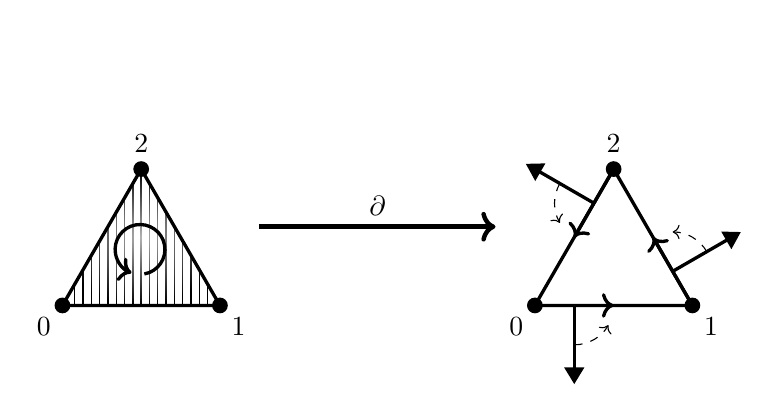
\begin{tikzpicture}[scale=2]
\tikzfading[name=fade outside,inner color=transparent!30,outer color=transparent!100]
\fill[pattern={Lines[angle=90, yshift=4pt, line width=.5pt]}](0,0) -- ++(60:1) -- ++(-60:1) -- cycle;
\fill[white,path fading=fade outside](0,0) -- ++(60:1) -- ++(-60:1) -- cycle;
\draw[very thick] (0,0) node[below left=.3pt]{$0$} -- ++(60:1) node[above=2pt]{$2$} -- ++(-60:1)node[below right=.3pt]{$1$} -- cycle;
\draw[very thick,->] (0.52,.2) arc[start angle=-80, end angle=250, radius=4.5pt];
\fill (0,0) circle (.05) -- ++(60:1) circle (.05) -- ++(-60:1) circle (.05);
\draw[ultra thick,->] (1.25,0.5) -- (2.75,.5) node[midway,above]{$\partial$} ;
\draw[very thick] (3,0) node[below left=.3pt]{$0$} -- ++(60:1) node[above=2pt]{$2$} -- ++(-60:1)node[below right=.3pt]{$1$} -- cycle ;
\fill (3,0) circle (.05) -- ++(60:1) circle (.05) -- ++(-60:1) circle (.05);
\draw[very thick,->] (3,0) -- (3.5,0);
\draw[very thick,->] (4,0) -- +(120:.5);
\draw[very thick,->] ($(3,0)+(60:1)$) -- ($(3,0)+(60:.5)$);

\begin{scope}[>=Triangle]
\draw[very thick,->] (3.25,0) -- (3.25,-.5);
\draw[very thick,->] ($(4,0)+(120:.25)$) -- ($(4,0)+(120:.25)+(30:.5)$);
\draw[very thick,->] ($(4,0)+(120:1)+(-120:.25)$) -- ($(4,0)+(120:1)+(-120:.25)+(150:.5)$);
\end{scope}

\draw[dashed,->] (3.25,-.25) arc[start angle=-90, end angle=-30, radius=.25];
\draw[dashed,->] ($(4,0)+(120:.25)+(30:.25)$) arc[start angle=30, end angle=90, radius=.25];
\draw[dashed,->] ($(4,0)+(120:1)+(-120:.25)+(150:.25)$) arc[start angle=150, end angle=210, radius=.25];
\end{tikzpicture}
\caption{The orientation of the boundary.}\label{fig:orientation}
\end{figure}
\end{defi}

These boundary morphisms satisfy the well known property that if $e^p$ is a codimension~$2$ face of some cell $e^{p+2}$ and $e^{p+1}_1,e^{p+1}_2$ denote the two codimension~1 faces of $e^{p+2}$ adjacent to $e^p$ then the two compositions of boundary morphisms $\Z(e^{p+2})\rightarrow \Z(e_1^{p+1}) \rightarrow \Z(e^p)$ and $\Z(e^{p+2})\rightarrow \Z(e_2^{p+1}) \rightarrow \Z(e^p)$ are opposite of each other. In particular, composing boundary morphisms between oriented coefficients does not define a cellular cosheaf.

\begin{defi}[Dihomologic Orientations]\label{definition:rel_or}
Let $\epsilon$ be the dihomologic pseu\-do-cell associated with an adjacent pair $e^p\leq e^q$, we define its \emph{group of oriented coefficients} to be:
\begin{equation*}
\Z(\epsilon)=\Z(e^p;e^q):=\Hom(\Z(e^p);\Z(e^q)).
\end{equation*}
We call a generator of such group an \emph{orientation} of $\epsilon$ or a \emph{relative orientation} of the pair $e^p\leq e^q$ and denote such an element by the symbol $[e^p; e^q]$. If $\epsilon'$ is a codimension~1 face of the pseudo-cell $\epsilon$, we also have a \emph{boundary morphism} $\Z(\epsilon)\rightarrow \Z(\epsilon')$ defined by the boundary morphisms between the groups of oriented coefficients of cells of $K$ and, up to sign, by the functorial properties of $\Hom$. They are shown in the diagram below.
\begin{equation}
\tag{D2}\label{diag:bound_mor}
\begin{tikzcd}
& \Z\left(e^p;e^q\right) \arrow[ld,"(-1)^{p+1}\Hom(\partial\,;\,\id)" above left] \arrow[rd,"(-1)^p\Hom(\id\,;\,\partial')" above right] & & \Z\left(e^{p+1}\right)\arrow[d,"\partial" left] & \Z\left(e^q\right) \arrow[d,"\partial'" right] \\ \Z\left(e^{p+1};e^q\right) & & \Z\left(e^p;e^{q-1}\right) & \Z\left(e^p\right) & \Z\left(e^{q-1}\right)
\end{tikzcd}
\end{equation}
\end{defi}

Note that if $\epsilon$ is a dihomologic pseudo-cell of dimension $k$, its closure can be expressed as the cone over a space that has the homology of a $(k-1)$-sphere. In this description, $\epsilon$ corresponds to the open cone. Therefore, the singular homology of $\bar{\epsilon}$ relatively to $\bar{\epsilon}\setminus\epsilon$ is isomorphic to the singular homology of a $k$-ball relatively to its boundary. Thus, we could equivalently define $\Z(\epsilon)$ to be $H_k(\bar{\epsilon};\bar{\epsilon}\setminus\epsilon;\Z)$ as in the case of a regular CW-complex. Indeed, if $e^p\leq e^q$ is the indexing pair of the pseudo-cell $\epsilon$, there is a canonical isomorphism between the groups $H_{q-p}(\bar{\epsilon};\bar{\epsilon}\setminus\epsilon;\Z)$ and $\Hom(\Z(e^p);\Z(e^q))$. If we represent a cell $e^p$ by a $p$-dimensional real vector space inside a $q$-dimensional vector space (representing $e^q$) then the dihomologic pseudo-cell $\epsilon$ indexed by $e^p\leq e^q$ represents a supplementary sub-space of the former in the latter. An orientation of such supplementary space allows by wedge product to orient the $q$-dimensional vector space from an orientation of the $p$-dimensional one. The situation is explained by the cohomological bilinear cup product:
\begin{equation*}
\cup : H^p\left(\bar{e}\,^p;\bar{e}\,^p\setminus e^p\right)\otimes H^{q-p}\left(\bar{\epsilon};\bar{\epsilon}\setminus\epsilon\right) \rightarrow H^q\left(\bar{e}\,^q;\bar{e}\,^q\setminus e^q\right).
\end{equation*}
It is non-degenerate. To see it one can notice that all the spaces considered are supports of simplicial complexes so each of these groups can be computed simplicially. A generator of $H^p(\bar{e}\,^p;\bar{e}\,^p\setminus e^p)$ is represented by the simplicial cocycle whose value is $1$ on the barycentric simplex indexed by a complete flag $e^0<\dots<e^p$ and $0$ elsewhere. Likewise, a generator of $H^{q-p}(\bar{\epsilon};\bar{\epsilon}\setminus\epsilon)$ is represented by the simplicial cocycle whose value is $1$ on the barycentric simplex indexed by a complete flag $e^p<\dots<e^q$ and $0$ elsewhere. Their cup product is the simplicial cocycle whose value is $1$ on the barycentric simplex indexed by the complete flag $e^0<\dots<e^p<\dots<e^q$ and $0$ elsewhere. It represents a generator of $H^q(\bar{e}\,^q;\bar{e}\,^q\setminus e^q)$. It gives rise to an isomorphism:
\begin{equation*}
H^{q-p}(\bar{\epsilon};\bar{\epsilon}\setminus\epsilon)\cong \Hom\Big(H^p\left(\bar{e}\,^p;\bar{e}\,^p\setminus e^p\right);H^q\left(\bar{e}\,^q;\bar{e}\,^q\setminus e^q\right)\Big).
\end{equation*}
Using the universal coefficients theorem~\cite[Theorem~3.3 p.~113]{Car-Eil_hom_alg}
%\footnote{H. Cartan and S. Eilenberg. \emph{Homological Algebra}, .}
three times this isomorphism becomes:
\begin{equation*}
\Z(\epsilon) \cong \Hom\Big(\Hom\Big(\Hom(\Z(e^p);\Z);\Hom(\Z(e^q);\Z)\Big);\Z\Big).
\end{equation*}
Since all the groups involved are free, we can compose it with the musical isomorphism of the trace scalar product:
\begin{multline*}
\Hom\Big(\Hom\Big(\Hom(\Z(e^p);\Z);\Hom(\Z(e^q);\Z)\Big);\Z\Big)\\
\cong \Hom\Big(\Hom(\Z(e^q);\Z);\Hom(\Z(e^p);\Z)\Big),
\end{multline*}
and then with the transposition:
\begin{equation*}
\Hom\Big(\Hom(\Z(e^q);\Z);\Hom(\Z(e^p);\Z)\Big) \cong \Hom\Big(\Z(e^p);\Z(e^q)\Big),
\end{equation*}
to finally find our desired isomorphism $\Z(\epsilon)\cong\Hom(\Z(e^p);\Z(e^q))$. Note that the signs in the Definition~\ref{definition:rel_or}, diagram~\eqref{diag:bound_mor}, of the boundary morphisms between the groups of oriented coefficients of dihomologic pseudo-cells come from this description and the relations:
\begin{equation*}
d_1\alpha\cup\beta+(-1)^p\alpha\cup d_2\beta = 0 \textnormal{ and } d_3(\alpha\cup \gamma)=0+(-1)^p\alpha\cup d_4\gamma,
\end{equation*}
that come from the graded Leibniz rule. They are satisfied by all $\alpha\in H^p(\bar{e}\,^p;\bar{e}\,^p\setminus e^p)$, $\beta\in H^{q-p-1}(\bar{\epsilon}_1;\bar{\epsilon}_1\setminus\epsilon_1)$ and $\gamma\in H^{q-p-1}(\bar{\epsilon}_2;\bar{\epsilon}_2\setminus\epsilon_2)$, where:
\begin{enumerate}
\item $\epsilon_1$ and $\epsilon_2$ are adjacent dihomologic pseudo-cells respectively indexed by the pairs $e^{p+1}\leq e^q$ and $e^p\leq e^{q-1}$;
\item $d_1$ and $d_3$ are respectively transpose of the orientation boundary morphisms $\partial_1:\Z(e^{p+1})\rightarrow\Z(e^p)$ and ${\partial_3:\Z(e^{q})\rightarrow\Z(e^{q-1})}$;
\item $d_2:H^{q-p-1}(\bar{\epsilon}_1;\bar{\epsilon}_1\setminus\epsilon_1)\rightarrow H^{q-p}(\bar{\epsilon}_3;\bar{\epsilon}_3\setminus\epsilon_3)$ and $d_4:H^{q-p-1}(\bar{\epsilon}_2;\bar{\epsilon}_2\setminus\epsilon_2)\rightarrow H^{q-p}(\bar{\epsilon}_3;\bar{\epsilon}_3\setminus\epsilon_3)$ where $\epsilon_3$ is indexed by the pair $e^p\leq e^q$.
\end{enumerate}
If $[e^p]\in\Z(e^p)$ is an orientation of $e^p$ and $[e^p;e^q]\in\Z(e^p;e^q)$ is a relative orientation, we denote by $[e^p][e^p;e^q]$ the associated orientation of $e^q$. For all pairs $e^p\leq e^{p+1}$ of relative codimension~$1$, the inverse of the boundary morphism $\partial : \Z(e^{p+1})\rightarrow\Z(e^{p})$ defines a canonical relative orientation. We will always denote it by the symbol $[e^p;e^{p+1}]$ but we should emphasise that for any other positive dimensional dihomologic pseudo-cell the similar notation denotes an arbitrary orientation, possibly subject to conditions, as there are no canonical orientation for them. We can compose relative orientations in their morphism representations, we adopt the convention $[e^p;e^q][e^q;e^r]$ to denote $[e^q;e^r]\circ[e^p;e^q]$. In these notations, one can rewrite the anti-commutativity of the boundary morphisms as follows: for all adjacent pairs $e^p\leq e^{p+2}$ of relative codimension~$2$ we have:
\begin{equation*}
\sum_{e^p\,\leq\,e^{p+1}\,\leq\,e^{p+2}}\left[e^p;e^{p+1}\right]\left[e^{p+1};e^{p+2}\right]=0.
\end{equation*}

\begin{defi}[Cellular Chain and Cochain Complexes]
Let $F$ be a cellular cosheaf on $K$ and $k\in \N$. We define the group of \emph{cellular $k$-chains} of $K$ with coefficients in $F$ to be:
\begin{equation*}
C_k(K;F):=\bigoplus_{\dim e = k} F(e)\otimes_\Z\Z(e).
\end{equation*}
Moreover, if $[e]$ is an oriented $k$-cell of $K$ and $c$ is a $k$-chain with coefficients in $F$ we denote by $\langle c,[e]\rangle$ the unique element of $F(e)$ satisfying $c_e=\langle c,[e]\rangle\otimes [e]$. We also define the \emph{boundary operator} $\partial : C_k(K;F) \rightarrow C_{k-1}(K;F)$ by the formula:
\begin{equation*}
\partial f :=\sum_{e^{k-1}\,<\,e^k} \left\langle f,[e^k]\right\rangle\big|^{e^k}_{e^{k-1}}\otimes \left[e^{k-1}\right],
\end{equation*}
for all $f\in F(e^k)\otimes_\Z\Z(e^k)$ where $[e^{k-1}]$ is the image of $[e^k]$ by the boundary morphism. This relation can be written as ${[e^{k-1}][e^{k-1};e^k]=[e^k]}$ where $[e^{k-1};e^k]$ is the canonical relative orientation. The anti-commutativity of the boundary morphisms between oriented coefficients implies that $\partial^2=0$. Thus $(C_k(K;F);\partial)_{k\,\geq\,0}$ is a chain complex.

%\vspace{5pt}

Dually, when $F$ is a cellular sheaf, we have a \emph{cochain complex} with coefficients in $F$. For all $k\in \N$, the group of \emph{cellular $k$-cochains} is given by:
\begin{equation*}
C^k(K;F):= \prod_{\dim e = k} \Hom(\Z(e);F(e)).
\end{equation*}
For all $k$-cochains $\alpha$ with coefficients in $F$ and all oriented $k$-cells $[e]$, we denote by $\alpha[e]\in F(e)$ the value of the $e$-component of $\alpha$ evaluated at $[e]$. The \emph{coboundary operator} or \emph{differential} $\df:C^k(K;F)\rightarrow C^{k+1}(K;F)$ is given for all $k$-cochains $\alpha$ and all oriented $(k+1)$-cells $[e^{k+1}]$ by:
\begin{equation*}
\df\alpha\left[e^{k+1}\right]=\sum_{e^k\,<\,e^{k+1}}\alpha\left[e^k\right]\big|^{e^{k+1}}_{e^k},
\end{equation*}
where $[e^k]$ denotes the only orientation of $e^k$ whose image by the boundary morphism is $[e^{k+1}]$, i.e. $[e^k][e^k;e^{k+1}]=[e^{k+1}]$.

%\vspace{5pt}

The last cochain complex we define here is the complex of \emph{cellular cochains with compact support}. It is a sub-complex of $(C^k(K;F);\df)_{k\,\geq \,0}$ whose groups are given for all $k\in \N$, by:
\begin{equation*}
C_c^k(K;F):=\bigoplus_{\dim e = k} \Hom(\Z(e);F(e)).
\end{equation*}
The image of $C_c^k(K;F)$ under $\df$ is contained in $C_c^{k+1}(K;F)$ only because we assumed $K$ to be locally finite. A morphism of cosheaves or sheaves gives rise to a morphism of chain or cochain complexes, respectively. In a more categorical language, the association $F\mapsto (C_k(K;F);\partial)_{k\,\geq\,0}$ for $F$ a cosheaf and $G\mapsto (C_{(c)}^k(K;G);\df)_{k\,\geq\,0}$ for $G$ a sheaf are covariant functors.
\end{defi}

\begin{defi}[Dihomologic chain complex]
Let $F$ be a dihomologic cellular cosheaf on $K$. We define the group of \emph{dihomologic cellular $k$-chains} of $K$ with coefficients in $F$ to be:
\begin{equation*}
\Omega_k(K;F):=\bigoplus_{\dim \epsilon = k} F(\epsilon)\otimes_\Z\Z(\epsilon),
\end{equation*}
If $[\epsilon]$ is an oriented $k$-pseudo-cell of $K$ and $c$ a $k$-chain with coefficients in $F$ we denote by $\langle c,[\epsilon]\rangle$ the unique element of $F(\epsilon)$ satisfying $c_\epsilon=\langle c,[\epsilon]\rangle\otimes [\epsilon]$. We also define the \emph{boundary operator} $\partial : \Omega_k(K;F) \rightarrow \Omega_{k-1}(K;F)$ by the formula:
\begin{equation*}
\partial \big(f\otimes[\epsilon^k]\big) :=\sum_{\epsilon^{k-1}\,<\,\epsilon^k} \left\langle f,[\epsilon^k]\right\rangle\big|^{\epsilon^k}_{\epsilon^{k-1}}\otimes \left[\epsilon^{k-1}\right],
\end{equation*}
for all $f\otimes[\epsilon^k] \in F(\epsilon^k)\otimes_\Z\Z(\epsilon^k)$, where $[\epsilon^{k-1}]$ is the image of $[\epsilon^k]$ by the boundary morphism.
\end{defi}

\begin{rema}
If the dihomologic pseudo-subdivision of $K$ is a regular subdivision of $K$ the last definition is identical to the definition of the cellular chain complex with coefficients in a cellular cosheaf on a CW-complex.
\end{rema}

\begin{defi}
Let $F$ be a cellular cosheaf (resp. a cellular sheaf). We define its \emph{homology} (resp. \emph{cohomology}, resp. \emph{cohomology with compact support}) to be the homology of its cellular chain complex (resp. cohomology of its cellular cochain complex, resp. cohomology of its cellular cochain complex with compact support). We also define the homology of a dihomologic cosheaf to be the homology of the associated chain complex.
\end{defi}

\begin{exam}
Given two sub-complexes $K_1\leq K_2$ of $K$ and an Abelian group~$G$, the homology of $[K_2;K_1;G]$ is exactly the same as the cellular homology of $K_2$ relatively to $K_1$ with coefficients in $G$.
\end{exam}

The following propositions illustrate the usefulness of these cellular constructions:

\begin{prop}
If $F$ is a sheaf of Abelian groups on $|K|$, constructible with respect to the skeletal filtration, then the sheaf cohomology of $F$ is isomorphic to the cellular cohomology of the cellular sheaf associated to $F$.
\end{prop}

The proof of this fact is easily derived from the fact that the open cover of $|K|$ by the open stars of its vertices is a Leray cover for $F$ and that the cellular cochain complex of its associated cellular sheaf is the complex of its \v Cech cochains, see~\cite[Théorème~5.10.1 p.~228]{God_top_alg}
%\footnote{R. Godement. \emph{Topologie Algébrique et Théorie des Faisceaux}, .}
for instance.

\begin{prop}
Whenever $F$ is the cellular cosheaf arising from a local system of coefficients $L$ on $|K|$ there is a canonical isomorphism from the cellular homology of $F$ to the singular homology of $|K|$ with coefficients in $L$.
\end{prop}

The result follows directly from the description in~\cite[Section~3.H. Local Coefficients pp.~327-337.]{Hat_alg_top}
%\footnote{A. Hatcher. \emph{Algebraic Topology}, }
of the complex of singular chains with coefficients in $L$ and an adaptation of the classical proof relating singular homology and cellular homology.

\begin{prop}
Let $K'$ be a subdivision of $K$ and $F$ be a cellular cosheaf on $K$. If $F'$ denotes the subdivision of $F$ we have the following injective morphism of chain complexes:
\begin{equation*}
\begin{array}{rcl}
C_k(K;F) & \longrightarrow & C_k(K';F') \\%
c & \longmapsto & \displaystyle \sum_{e^k\,\in\,K} \left(\;\sum_{\substack{e'^k\,\subset\,e^k\\ e'^k\,\in\,K'}} \left\langle c\,;\,[e^k]\right\rangle\otimes [e'^k]\; \right)
\end{array}
\end{equation*}
where the orientations are defined as follows: if $[e^k]$ is an orientation of $e^k$ then $[e'^k]$ is the image of such orientation under the isomorphism $H_k(\bar{e}\,^k;\bar{e}\,^k\setminus e^k)\rightarrow H_k(\bar{e}'^k;\bar{e}'^k\setminus e'^k)$ inverse of the map induced by the inclusion $({\bar{e}'^k\setminus e^k};\bar{e}'^k)\subset(\bar{e}\,^k\setminus e'^k;\bar{e}\,^k)$. This is a quasi-isomorphism of chain complexes.
\end{prop}

A proof of this can be found in~\cite[Theorem~1.5.2 p.~31]{She_cel_des}
%\footnote{A. Shepard. \emph{A Cellular Description of the Derived Category of a Stratified Space},.}
in the dual context of cellular sheaves. The same proposition holds for dihomologic subdivisions of cellular cosheaves on $K$. A proof of the specific case of the constant sheaf on the dihomologic subdivision is given in~\cite[Theorem~1.2 p.~12]{For_comb_nov}.
%\footnote{R. Forman, \emph{Combinatorial Novikov--Morse Theory}, .}

\begin{prop}
Let $F$ be a cellular cosheaf on $K$. If $F'$ denotes the dihomologic subdivision of $F$ we have the following injective morphism of chain complexes:
\begin{align*}
C_k(K;F) & \longrightarrow  \Omega_k(K;F') \\
c & \longmapsto  \sum_{e^0\,\leq\,e^k} \left\langle c\,;\,[e^k]\right\rangle\otimes \left[e^0;e^k\right]
\end{align*}
where the orientations are defined as follows: if $[e^k]$ is an orientation of $e^k$ then $[e^0;e^k]$ is the relative orientation defined by the relation $[e^0][e^0;e^k]=[e^k]$ where $[e^0]$ is the canonical orientation of the vertex $e^0$ of $K$. This is a quasi-isomorphism of chain complexes.
\end{prop}

This is an adaptation of the proof given by R. Forman.

\begin{proof}
Let us denote by $f$ the morphism of chain complexes given in the statement of the proposition. For all $q\in\N$, we have natural inclusions of the dihomologic complexes associated with the restrictions of $F'$ to the skeleta of $K$:
\begin{equation*}
\Omega_*\left(K^{(q)};F'\right)\subset \Omega_*\left(K^{(q+1)};F'\right).
\end{equation*}
We note that for every $k\in\N$, $f$ maps $C_k(K;F)$ to $\Omega_k(K^{(k)};F')$. Now we consider the spectral sequence associated with this filtration:
\begin{equation*}
E^r_{p,q}:=\frac{Z^r_{p,q} + \Omega_{q-p}\left(K^{(q-1)};F'\right)}{\partial Z^{r-1}_{p+r-2,q+r-1}+\Omega_{q-p}\left(K^{(q-1)};F'\right)}\;,
\end{equation*}
where $Z^r_{p,q}=\{c\in \Omega_{q-p}(K^{(q)};F') \,|\, \partial c \in \Omega_{q-p-1}(K^{(q-r)};F') \}$. The boundary operator $\partial^r_{p,q}:E^r_{p,q}\rightarrow E^r_{p-r+1,q-r}$ applied to an element $c\in E^r_{p,q}$ is given by computing $\partial c'\in \Omega_{q-p-1}(K;F')$ for any lift $c'\in Z^r_{p,q}$ and then projecting to $E^r_{p-r+1,q-r}$. The term $E^0_{p,q}$ is written as:
\begin{equation*}
E^0_{p,q}=\bigoplus_{e^p\,\leq\,e^q} F'(e^p;e^q)\otimes\Z(e^p;e^q),
\end{equation*}
where $F'(e^p;e^q)=F(e^q)$ by assumption. The boundary $\partial^0_{p,q}$ acts on the element $v\otimes[e^p;e^q]$ of the group $F'(e^p;e^q)\otimes\Z(e^p;e^q)=F(e^q)\otimes\Z(e^p;e^q)$ as follows:
\begin{equation*}
\partial^0_{p,q} \left(v\otimes[e^p;e^q]\right) =\sum_{e^p\,\leq\,e^{p+1}\,\leq \,e^q}v\otimes \left[e^{p+1};e^q\right] \in \bigoplus_{e^p\,\leq\,e^{p+1}\,\leq \,e^q}F'\left(e^{p+1};e^q\right)\otimes\Z\left(e^{p+1};e^q\right),
\end{equation*}
where $[e^{p+1};e^q]$ is the image of $[e^p;e^q]$ by the boundary $\partial:\Z(e^{p};e^q)\rightarrow \Z(e^{p+1};e^q)$. This morphism is given by $(-1)^{p+1}\Hom(\partial';\id)$ with $\partial':\Z(e^{p+1})\rightarrow\Z(e^q)$. Therefore, if we decide to write $[e^p;e^q]$ in the form $\alpha\otimes[e^q]\in \Hom(\Z(e^p);\Z)\otimes \Z(e^q)$ we have $[e^{p+1};e^q]=(-1)^{p+1}(\alpha\circ\partial')\otimes[e^q]$. As a consequence, we see that the line of index $q$ of the $E^0$-page of the spectral sequence splits into the direct sum of the cellular cochain complexes of the $K(e^q)$'s with coefficients in the constant cellular sheaves $F(e^q)\otimes\Z(e^q)$ with coboundary operator $\df$ twisted by $(-1)^{p+1}$:
\begin{equation*}
\begin{tikzcd}
\cdots \longrightarrow E^0_{p,q} \ar[rr,"\partial^0"] & & E^0_{p+1,q} \longrightarrow \cdots \\%
\displaystyle \bigoplus_{e^q\,\in\,K} C^p\big(K(e^q);F(e^q)\otimes\Z(e^q)\big) \ar[rr,"\oplus(-1)^{p+1}\df" below] & & \displaystyle \bigoplus_{e^q\,\in\,K} C^{p+1}\big(K(e^q);F(e^q)\otimes\Z(e^q)\big)
\end{tikzcd}
\end{equation*}
Since the support of $K(e^q)$ is the closure of $e^q$, the $E^1$-page of the spectral sequence is concentrated on the $0^{\rm th}$ column and satisfies:
\begin{equation*}
E^1_{0,q}=\bigoplus_{e^q\,\in\,K} H^0\big(K(e^q);F(e^q)\otimes\Z(e^q)\big).
\end{equation*}
We note that $E^1_{0,q}\subset E^0_{0,q}$ and is precisely the image of $f$. It defines an isomorphism between this $0^{\rm th}$ column and $C_*(K;F)$ and therefore between the homology of $F$ and the homology of its subdivision $F'$. Moreover, we deduce that our filtration is adapted to the cokernel of $f$ and that computing the first page of the induced spectral sequence amounts to replace in our computations the cohomology groups of the $K(e^q)$'s with coefficients in the group $F(e^q)\otimes\Z(e^q)$ with their reduced cohomology groups. Since the $|K(e^q)|$'s are contractible, they all vanish. Thus, the cokernel of $f$ has trivial homology and $f$ is a quasi-isomorphism.
\end{proof}

\section{A Poincaré--Lefschetz Theorem for Dihomologic Cellular Cosheaves}

Let $K$ be a locally finite regular CW-complex and $F$ be a dihomologic cosheaf on~$K$. The chain complex $(\Omega_k(K;F);\partial)_{k\,\geq\,0}$ is actually the total complex of a bicomplex. The $k$-dimensional dihomologic pseudo-cells are represented by adjacent pairs of cells $e^p\leq e^q$ with $q-p=k$. Hence, their set is partitioned into sets of pseudo-cells of different types. If we say that a dihomologic pseudo-cell indexed by $e^p\leq e^q$ has type $(p,q)$, the set of $k$-dimensional dihomologic pseudo-cells is the disjoint union of the set of pseudo-cells of type $(p,q)$ for all $q-p=k$. Similarly the group $\Omega_k(K;F)$ splits into the following direct sum:
\begin{equation*}
\Omega_k(K;F)=\bigoplus_{q-p=k}\Omega_{p,q}(K;F),
\end{equation*}
where:
\begin{equation*}
\Omega_{p,q}(K;F):=\bigoplus_{e^p\,\leq \,e^q}F(e^p;e^q)\otimes\Z(e^p;e^q),
\end{equation*}
for all $p,q\in\N$. A codimension~$1$ face of $e^p\leq e^q$ either starts with $e^p$ or ends with $e^q$ and therefore the restriction of the boundary operator to $\Omega_{p,q}(K;F)$ takes its values in the sum $\Omega_{p+1,q}(K;F)\oplus\Omega_{p,q-1}(K;F)$. The operator $\partial$ is the sum of an operator $\partial_1$ of bidegree $(+1;0)$ and an operator $\partial_2$ of bidegree $(0;-1)$. With this additional structure, we can consider the two canonical filtrations and associated spectral sequences. We will only look at the (decreasing) horizontal filtration, that is to say, the one filtered by the index $p$. The filtering pieces are, for all $k,l\in\N$:
\begin{equation*}
\Omega_k^{(l)}(K;F):=\bigoplus_{\substack{q-p=k\\ p\,\geq\,l}}\Omega_{p,q}(K;F).
\end{equation*}
The associated spectral sequence is given for all $p,q\in\Z$ by:
\begin{equation*}
E^r_{p,q}:=\frac{Z^r_{p,q} + \Omega_{q-p}^{(p+1)}(K;F)}{\partial Z^{r-1}_{p-r+1,q-r+2}+\Omega_{q-p}^{(p+1)}(K;F)},
\end{equation*}
where $Z^r_{p,q}$ denotes $\{c\in \Omega_{q-p}^{(p)}(K;F) \,|\, \partial c \in \Omega_{q-p-1}^{(p+r)}(K;F) \}$. The boundary operator $\partial^r_{p,q}:E^r_{p,q}\rightarrow E^r_{p+r,q+r-1}$ applied to an element $c\in E^r_{l,k}$ is given by computing $\partial c'\in \Omega^{(p+r)}_{q-p-1}(K;F)$ for any lift $c'\in Z^r_{p,q}$ and then projecting to $E^r_{p+r,q+r-1}$.

\begin{prop}\label{prp:degenerate_E2_lef}
If there is an $n\in\N$ such that for every cell $e$ of $K$ the local cosheaf $F_e$ has its homology concentrated in dimension $n$ then the horizontal spectral sequence of $\Omega(K;F)$ degenerates at the second page.
\end{prop}

\begin{proof}
We have:
\begin{equation*}
E^0_{p,q}\cong \Omega_{p,q}(K;F),
\end{equation*}
and $\partial^0_{p,q}$ corresponds to the vertical component, $\partial_2$, of the total boundary operator, $\partial$, of $(\Omega_{k}(K;F);\partial)_{k\,\in\,\N}$. The following page $(E^1_{p,q})_{p,q\,\in\,\N}$ is given by the homology groups of the column complexes of the bicomplex $(\Omega_{p,q}(K;F);\partial_1;\partial_2)_{p,q\,\in\,\N}$. Let $p,q\in\N$ and let's consider the morphism:
\begin{equation*}
\Phi_{p,q} : \Omega_{p,q}(K;F) \rightarrow \bigoplus_{e^p\,\in\,K}\Hom\big(\Z(e^p);C_q(K;F_{e^p})\big),
\end{equation*}
for which the $(e^p)$-component of the image of an element $c$ is given by the linear map:
\begin{equation*}
[e^p]\mapsto (-1)^{\frac{p(p+1)}{2}+\frac{q(q+1)}{2}}\sum_{e^q\,>\,e^p}\langle c,[e^p;e^q]\rangle\otimes[e^q],
\end{equation*}
where $[e^p;e^q],[e^q]$ are some choices of orientations satisfying $[e^p][e^p;e^q]=[e^q]$ (the map does not depend on such choices). For a fixed $p\in\N$, the collection $(\Phi_{p,q})_{q\,\in\,\N}$ is almost a chain complex isomorphism between the $p^{\rm th}$ column of the bicomplex of $F$-valued dihomologic chains $(\Omega_{p,q}(K;F);\partial_2)_{q\,\geq\,0}$ and the direct sum over the $p$-cells $e^p$ of the complexes $(\Hom(\Z(e^p);C_q(K;F_{e^p}));\Hom(\Z(e^p);\partial))_{q\,\geq\,0}$. We have $\partial\Phi_{p,q}=(-1)^{q-p}\Phi_{p,q-1}\partial_2$ so $(\Phi_{p,q})_{q\,\in\,\N}$ still defines an isomorphism in homology. Each of the $\Phi_{p,q}$ being individually an isomorphism is a matter of bookkeeping. On the left hand side we sum the groups $F(e^p,e^q)\otimes \Z(e^p,e^q)$ over all ordered pairs of cells $e^p\leq e^q$ and on the right hand side we sum the groups $\Hom(\Z(e^p);F(e^p,e^q)\otimes\Z(e^q))$ over the same index set but in a different order, $\Phi_{p,q}$ then sends bijectively each one of the former summands to one of the latter summands by means of the composition:
\begin{multline*}
F(e^p,e^q)\otimes \Z(e^p,e^q)\\
=
%\begin{tikz}
 F(e^p,e^q)\otimes \Hom(\Z(e^p);\Z(e^q))
% \arrow[r,"\pm 1" above] &
\arr\Hom(\Z(e^p);F(e^p,e^q)\otimes\Z(e^q)).
%\end{tikz}
\end{multline*}
Let us now prove the claim about the ``commutativity'' relation with the boundary operators. Let $c$ be a chain of type $(p;q)$. On the one hand, for all $p$-cells $e^p$ of $K$, the value of the $(e^p)$-component of $\Phi_{p,q-1}(\partial_2 c)$ on an orientation $[e^p]$ is given by the following formula:
\begin{equation*}
\Phi_{p,q-1}(\partial_2c)[e^p]=(-1)^{\frac{p(p+1)}{2}+\frac{q(q-1)}{2}}\sum_{e^{q-1}\,>\,e^p}\left(\sum_{e^q\,>\,e^{q-1}} \left\langle c, [e^p;e^q]\right\rangle \Big|^{e^p,e^q}_{e^p,e^{q-1}}\right)\otimes\left[e^{q-1}\right],
\end{equation*}
where $[e^p][e^p,e^{q-1}]=[e^{q-1}]$ and $[e^p,e^q]=(-1)^p[e^p,e^{q-1}][e^{q-1},e^q]$. That is to say:
\begin{equation*}
\Phi_{p,q-1}(\partial_2c)[e^p]=(-1)^{\frac{p(p-1)}{2}+\frac{q(q-1)}{2}}\sum_{e^{q-1}\,>\,e^p}\left(\sum_{e^q\,>\,e^{q-1}} \left\langle c, [e^p;e^q]\right\rangle \Big|^{e^p,e^q}_{e^p,e^{q-1}}\right)\otimes\left[e^{q-1}\right],
\end{equation*}
where $[e^p][e^p,e^q]=[e^{q-1}][e^{q-1},e^q]$. Since we changed the equation defining the orientation, we had to compensate with the multiplication by a factor $(-1)^p$ which turned $(-1)^{\frac{p(p+1)}{2}}$ into $(-1)^{\frac{p(p-1)}{2}}$. On the other hand, the value of the $(e^p)$-component of $\partial\Phi_{p,q}(c)$ on $[e^p]$ is the same as the boundary of $\Phi_{p,q}(c)[e^p]$:
\begin{align*}
\partial\Phi_{p,q}(c)[e^p] & =(-1)^{\frac{p(p+1)}{2}+\frac{q(q+1)}{2}} \sum_{e^q\,>\,e^p} \left(\sum_{e^{q-1}\,<\,e^q} \left\langle c,[e^p,e^q]\right\rangle \Big|^{e^q}_{e^{q-1}}\otimes\left[e^{q-1}\right] \right),
\end{align*}
where $[e^p][e^p;e^q]=[e^q]$ and $[e^{q-1}][e^{q-1};e^q]=[e^q]$, i.e. $[e^p][e^p,e^q]=[e^{q-1}][e^{q-1},e^q]$. The element $\langle c,[e^p,e^q]\rangle$ of $F(e^p,e^q)$ in the last formula is understood as an element of $F_{e^p}(e^q)$ hence we have to apply the extension morphisms of $F_{e^p}$ and this is why we wrote $\langle c,[e^p,e^q]\rangle |^{e^q}_{e^{q-1}}$. However, these extension morphisms are zero whenever $e^{q-1}$ doesn't contain $e^p$ and identical to those of $F$ in the opposite case. Therefore, we can write:
\begin{align*}
\partial\Phi_{p,q}(c)[e^p] & =(-1)^{\frac{p(p+1)}{2}+\frac{q(q+1)}{2}} \sum_{e^q\,>\,e^p} \left(\sum_{e^p\,<\,e^{q-1}\,<\,e^q} \left\langle c,[e^p,e^q]\right\rangle \Big|^{e^p,e^q}_{e^p,e^{q-1}}\otimes\left[e^{q-1}\right] \right) \\
& = (-1)^{\frac{p(p+1)}{2}+\frac{q(q+1)}{2}} \sum_{e^{q-1}\,>\,e^p}\left(\sum_{e^q\,>\,e^{q-1}} \left\langle c, [e^p;e^q]\right\rangle \Big|^{e^p,e^q}_{e^p,e^{q-1}}\right)\otimes\left[e^{q-1}\right] \\ & = (-1)^{q-p}\Phi_{p,q-1}(\partial_2c)[e^p].
\end{align*}
For each $p$-cell, the group $\Z(e^p)$ is free so the Universal Coefficient Theorem ensures that $E^1_{p,q}$ is isomorphic to the direct sum of the $\Hom(\Z(e^p);H_q(K;F_{e^p}))$'s. By assumptions, $H_q(K;F_{e^p})$ is trivial as soon as $q$ is not $n$. As a consequence, all pages following $E^1$ are concentrated on the horizontal line $\{q=n\}$. Since $\partial^r_{p,q}$ has bidegree $(r,r-1)$, the spectral sequence degenerates at the second page.
\end{proof}

\begin{defi}\label{def:loc_hom_shea}
Let $F$ be a dihomologic cosheaf of a regular CW-complex $K$ and $q$ be a non-negative integer. The $q^{\rm th}$ \emph{sheaf of local homology} of $F$ is denoted by $H_q(F_*)$. It is a cellular sheaf on $K$ and it is given by the groups:
\begin{equation*}
H_q(F_*):e^p\mapsto H_q(K;F_{e^p}).
\end{equation*}
Its restriction morphisms are induced in homology by the localisation morphisms $F_{e^{p_1}}\rightarrow F_{e^{p_2}}$ for all cells $e^{p_1}\leq e^{p_2}$.
\end{defi}
\begin{theo}[Cellular Poincaré--Lefschetz Theorem]\label{thm:cell_poinca_lef}
Let $K$ be a finite dimensional, locally finite and regular CW-complex, $n$ be a non-negative integer, and $F$ be a dihomologic cosheaf on $K$ whose sheaves of local homology $H_q(F_*)$ vanish for all $q\neq n$. Then for all integers $k$, $H_k(K;F)$ and $H_c^{n-k}(K;H_n(F_*))$ are canonically isomorphic. In particular, $H_k(K;F)$ vanishes for all $k>n$. If in addition $K$ has dimension $n$, then this isomorphism comes from an injective quasi-isomorphism:
\begin{equation*}
\big(C^{n-k}_c\big(K;H_n(F_*)\big);\df\big)_{k\,\geq\,0}\rightarrow \big(\Omega_k(K;F);\partial\big)_{k\,\geq\,0}.
\end{equation*}
\end{theo}
\begin{proof}
Let $d$ denote $\dim K$. We consider the horizontal filtration of the homology of $F$:
\begin{equation*}
0\subset H_k(K;F)^{(d)} \subset \cdots \subset H_k(K;F)^{(n-k)} \subset \cdots \subset H_k(K;F)^{(0)},
\end{equation*}
whose graded pieces:
\begin{equation*}
E^\infty_{d,k+d} \hspace{0.5cm} \cdots \hspace{0.5cm} E^\infty_{n-k,n} \hspace{0.5cm} \cdots \hspace{0.5cm} E^\infty_{0,k},
\end{equation*}
satisfy, in light of the last proposition, $E^\infty_{p,q}=E^2_{p,q}=0$ as soon as $q$ is different from $n$. Therefore, for all integers $k$, $H_k(K;F)=H_k(K;F)^{(n-k)}=E^\infty_{n-k,n}=E^2_{n-k,n}$. Now because of the isomorphisms $(\Phi_{p,q})_{p,q\,\in\,\N}$ given in the last proof, we recognise that $E^1_{p,q}\cong C^p_c(K;H_q(F_*))$. Then it remains only to show that the boundary operator $\partial^1_{p,q}$ of the spectral sequence is mapped to the coboundary operator $\df$. If $c'\in\Omega_{p,q}(K;F)$ is a $\partial_2$-cycle representing an element $c\in E^1_{p,q}$ then $\partial_1 c'$ is a $\partial_2$-cycle representing $\partial^1_{p,q} c$. We have:
\begin{equation*}
\left\langle \partial_1 c',[e^{p+1};e^q]\right\rangle = \sum_{e^p\,<\,e^{p+1}} \left\langle c',[e^{p};e^q]\right\rangle \Big|^{e^p,e^q}_{e^{p+1};e^q},
\end{equation*}
where $[e^{p};e^q]=(-1)^{p+1}[e^p;e^{p+1}][e^{p+1};e^q]$. Hence the image of $\partial_1 c'$ under $\Phi$ satisfies:
\begin{equation*}
\Phi_{p+1,q}(\partial_1 c')\left[e^{p+1}\right]=(-1)^{\frac{(p+2)(p+1)}{2}+\frac{q(q+1)}{2}} \sum_{e^q\,>\,e^{p+1}}\left(\sum_{e^p\,<\,e^{p+1}} \left\langle c',[e^{p};e^q]\right\rangle \Big|^{e^p,e^q}_{e^{p+1};e^q} \right)\otimes[e^q],
\end{equation*}
where $[e^{p+1}][e^{p+1};e^q]=[e^q]$ and $[e^{p};e^q]=(-1)^{p+1}[e^p;e^{p+1}][e^{p+1};e^q]$. Which can be written as:
\begin{equation*}
\begin{split}
\Phi_{p+1,q}(\partial_1 c')\left[e^{p+1}\right] & =(-1)^{\frac{p(p+1)}{2}+\frac{q(q+1)}{2}}\sum_{e^p\,<\,e^{p+1}}\left(\sum_{e^q\,>\,e^{p+1}} \left\langle c',[e^{p};e^q]\right\rangle \Big|^{e^p,e^q}_{e^{p+1};e^q} \otimes[e^q]\right) \\
& = (-1)^{\frac{p(p+1)}{2}+\frac{q(q+1)}{2}}\sum_{e^p\,<\,e^{p+1}} \Psi_{e^p}^{e^{p+1}} \left(\sum_{e^q\,>\,e^{p}} \left\langle c',[e^{p};e^q]\right\rangle \otimes[e^q]\right),
\end{split}
\end{equation*}
where $[e^{p+1}][e^{p+1};e^q]=[e^q]$, $[e^{p};e^q]=[e^p;e^{p+1}][e^{p+1};e^q]$, and $\Psi_{e^p}^{e^{p+1}}$ is the chain complex morphism associated with the cosheaf morphism $F_{e^p}\rightarrow F_{e^{p+1}}$. Therefore, $\Phi_{p+1,q}(\partial^1_{p,q} c)$ is the $(p+1)$-cochain with compact support that associates to an oriented cell $[e^{p+1}]$ the sum, over its codimension~1 faces, of the images in $H_q(K;F_{e^{p+1}})$ of the homology classes $[(-1)^{\frac{p(p+1)}{2}+\frac{q(q+1)}{2}} \sum_{e^q\,>\,e^{p}} \langle c',[e^{p};e^q]\rangle \otimes[e^q]]\in H_q(K;F_{e^{p}})$ where $[e^{p};e^q]=[e^p;e^{p+1}][e^{p+1};e^q]$ and $[e^{p};e^q]=[e^p;e^{p+1}][e^{p+1};e^q]$. Finally, this is precisely $\df\Phi_{p,q}(c)$ for:
\begin{equation*}
\df\Phi_{p,q}(c)[e^{p+1}]=\sum_{e^p\,<\,e^{p+1}}\Phi_{p,q}(c)[e^p],
\end{equation*}
where $[e^{p}][e^{p};e^{p+1}]=[e^{p+1}]$ and $\Phi_{p,q}(c)[e^p]=[(-1)^{\frac{p(p+1)}{2}+\frac{q(q+1)}{2}} \sum_{e^q\,>\,e^{p}} \langle c',[e^{p};e^q]\rangle\linebreak \otimes[e^q]]$.


To prove the second part of the statement, when $\dim K=n$, we need to remember that $\Phi$ provided us with an isomorphism between the chain complexes $(E^1_{n-k,n};\partial^1)_{k\,\geq\,0}$ and $(C^{n-k}_c(K;H_n(F_*));\df)_{k\,\geq\,0}$. Also, in the special context of spectral sequences of bicomplexes we know that $E^1_{n-p,n}$ is the $n^{\rm th}$ homology group of the $(n-k)^{\rm th}$ column of $(\Omega_{p,q}(K;F);\partial_1;\partial_2)_{p,q\,\geq\,0}$. With the dimensional assumption, this is the homology group of highest dimension and therefore the same as the group of cycles. We have an inclusion of $E^1_{n-k,n}$ in $\Omega_{n-k,n}(K;F)$ as the kernel of the vertical part of the boundary operator, namely $\partial_2$. With this description, it is clearly an injective morphism of chain complexes whose cokernel inherits a bicomplex structure. By construction, all the columns of this bicomplex are exact and so is its total complex. Our injective quasi-isomorphism is then the composition of $\Phi$ with the inclusion of $(E_{n-k,n};\partial^1)_{k\,\geq\,0}$ in the total complex $(\Omega_k(K;F);\partial)_{k\,\geq\,0}$.
\end{proof}

\begin{thebibliography}{Zee62a}
\bibitem[CE56]{Car-Eil_hom_alg} Cartan, Henri; Eilenberg, Samuel Homological Algebra, Princeton Mathematical Series, 19, Princeton University Press, 1956.
\bibitem[CF67]{Coo-Fin_hom_cel} Cooke, George E.; Finney, Ross L. Homology of Cell Complexes, Princeton University Press and the University of Tokyo Press, 1967.
\bibitem[Cur14]{Cur_she_cos} Justin Curry, Sheaves, Cosheaves and Applications, 2014, https://arxiv.org/abs/1303.3255v2.
\bibitem[For02]{For_comb_nov} Forman, Robin Combinatorial Novikov–Morse Theory, Int. J. Math., Volume 13 (2002) no. 4, pp. 333-368.
\bibitem[GS80]{Gal-Ste_Cla_Sim} Galewski, David E.; Stern, Ronald J. Classification of Simplicial Triangulations of Topological Manifolds, Ann. Math. (2), Volume 111 (1980) no. 1, pp. 1-34.
\bibitem[God58]{God_top_alg} Godement, Roger Topologie Algébrique et Théorie des Faisceaux, Publications de l’Institut de mathématique de l’Université de Strasbourg, 13, Hermann, 1958.
\bibitem[Hat02]{Hat_alg_top} Hatcher, Allen Algebraic Topology, Cambridge University Press, 2002.
\bibitem[Kas84]{Kas_rie_hil} Kashiwara, Masaki The Riemann–Hilbert Problem for Holonomic Systems, Publ. Res. Inst. Math. Sci., Volume 20 (1984) no. 2, pp. 319-365.
\bibitem[LW69]{Lun-Wei_top_cw} Lundell, Albert T.; Weingram, Stephen The Topology of CW Complexes, The University Series in Higher Mathematics, Van Nostrand Reinhold Co., 1969.
\bibitem[Mun84]{Munk_ele_alg} Munkres, James R. Elements of Algebraic Topology, Addison-Wesley Publishing Group, 1984.
\bibitem[She85]{She_cel_des} Shepard, Allan D. A Cellular Description of the Derived Category of a Stratified Space, Ph. D. Thesis, Brown University, Providence, USA (1985).
\bibitem[Whi39]{Whi_sim_spa} Whitehead, John H. C. Simplicial Spaces, Nuclei and m-Groups, Proc. Lond. Math. Soc. (2), Volume 45 (1939), pp. 243-327.
\bibitem[Whi49]{Whi_com_hom} Whitehead, John H. C. Combinatorial Homotopy. I, Bull. Am. Math. Soc., Volume 55 (1949), pp. 213-245.
\bibitem[Zee62a]{Zee_dih_i} Zeeman, Erik C. Dihomology I. Relations Between Homology Theories, Proc. Lond. Math. Soc. (3), Volume 12 (1962), pp. 609-638.
\bibitem[Zee62b]{Zee_dih_ii} Zeeman, Erik C. Dihomology II. The Spectral Theories of a Map, Proc. Lond. Math. Soc. (3), Volume 12 (1962), pp. 639-689.
\bibitem[Zee63]{Zee_dih_iii} Zeeman, Erik C. Dihomology III. A Generalization of the Poincaré Duality for Manifolds, Proc. Lond. Math. Soc. (3), Volume 13 (1963), pp. 155-183.
\end{thebibliography}
\end{document}
